%\section{Delta-kick dynamics}
\section{Introduction}

As mentioned in Sec.~\ref{ss:pert_opt_latt}, the use of optical lattice potentials is ubiquitous in the field of ultracold atoms. Given their near perfect periodic structure, it is interesting to examine the effect these lattices have on already periodic systems. For a rapidly rotating condensate, the density profile will feature a large periodic Abrikosov lattice having $6$-fold rotational symmetry i.e.\ a triangular lattice. The use of optical lattices stationary in the co-rotating frame on vortex lattices has previously been shown to allow for pinning of the vortex cores to the lattice maxima \cite{OL:Reijnders_prl_2004,Vtx:Tung_prl_2006}. Assuming blue detuned laser fields, the lattice maxima will drive atoms away, and make it favourable for vortex cores to sit in these positions. A transition between lattice geometries can be observed in these cases. This is, however, experimentally challenging as in the lab frame the optical lattice must rotate with the vortex lattice and match its rotation rate. Nevertheless, the creation of a rotating quasi two-dimensional optical lattice was achieved in~\cite{Vtx:Tung_prl_2006}, where the authors used a rotating mask with the holes placed in such a way as to allow for the required optical diffraction patterns. However, the system suffered from difficulties arising from the inclusion of a mechanically rotating stage, as well as the heating effects due to the presence of the always-on optical lattice. As the vortex lattice has 6-fold rotational symmetry, after rotating by
$\Omega_{k}=6\Omega\approx 2\pi\times 6$ Hz the system has returned to its initial orientation. It is therefore intriguing to see if the need for a rotating optical potential can be replaced by a periodically flashed optical lattice. Here, we will investigate the effect of a single application of an optical lattice to the vortex lattice.

 For short application times, the potential will kick the wavefunction, and can be seen as leaving a phase imprint with minimal immediate density change. As discussed in Sec.~\ref{ss:pert_opt_latt}, the effect of the kick can then be observed in the ensuing dynamics. Interestingly, one can observe the appearance of moir\'e interference patterns in the condensate density, while the positions of the vortex cores are only minimally affected. We will begin by discussing the model, and present the explanation of the resulting interference pattern. We will show that it stems from the interference between the different $\mathbf{k}$-vectors, with signatures of the effect being visible in the condensate's kinetic energy spectrum. Finally, we will discuss the uses of this effect as a microscope for observing the presence of vortex lattices without time-of-flight.

As already discussed in detail above, given the large number of vortices in the condensate density, as well as the lowered density resulting from the large centrifugal forces, the vortex cores become large and form a highly periodic triangular lattice. The non-orthogonal lattice vectors are given in position space by $\mathbf{a}_1 = a_v[1,0]$ and $\mathbf{a}_2 = a_v[-1/2, \sqrt{3}/2]$, where $a_v$ is the distance between vortex cores. The lattice ``constant'' is truly only constant in areas of near uniform density. Thus, due to the inhomogeneous wavefunction density, the vortices near the edges are separated by a larger distance than those at the centre. For the analysis we have therefore chosen to ignore all vortices near the condensate edge. The momentum space ($\mathbf{k}$-space) lattice vectors are reciprocal to the given $\mathbf{r}$-space vectors, and given by $\mathbf{b}_1 = 4\pi/(\sqrt{3}a_v)\left[\sqrt{3}/2,1/2\right]$ and $\mathbf{b}_2 = 4\pi/(\sqrt{3}a_v)\left[0,1\right]$.
%[!!!!check for consistency!!!!]

\section{Model}

Using an optical potential one can create a perturbation in the condensate density by switching it on for a brief period of time. Such a kick must occur only for a time much shorter than the rotation period of the vortex lattice, of angular rotation frequency $\Omega = 0.995\omega_\perp$, so that the effect is limited to a phase imprinting and not to a direct change in the density distribution. For the work carried out herein, the duration of the kick is $\tau_{\text{kick}}=10^{-5}$~s, which is fast compared to the classical rotation period of the 6-fold symmetric lattice of $T_{6} \approx 1.66\times 10^{-1}$~s. This ensures that the vortex lattice is essentially stationary during the kick. To examine the effect that periodicity plays on the system, the optical potential was chosen to match the geometry of the Abrikosov vortex lattice, with the angle of relative alignment $\theta_\Delta$ given as a free parameter. The optical potential was modelled as the sum of counter-propagating laser beams, as
\begin{equation}
    V_{\text{opt}} = V_0\displaystyle\sum_{j}\cos^2 \left[ \textbf{k}_{j}\cdot\textbf{r} \right],
\end{equation}
where $V_0$ is the optical lattice potential amplitude, and $j=[0,1,2,\ldots ]$ is the index of each respective laser with a differing $\mathbf{k}$-space wave-vector. By careful choice of the wave-vectors $\textbf{k}_{j}$ the density modulation given by the vortices is matched to the optical potential. This is achieved using the reciprocal lattice vectors defined by the vortex lattice, $\mathbf{b}_{1,2}$, and an additional third wave-vector, $\mathbf{k}_3 = 4\pi/(\sqrt{3}a_o)\left[\sqrt{3}/2,-1/2\right]$. For the resulting optical potential, we define the lattice sites as the maxima of intensity. These are in turn matched with the condensate density minima of the vortex lattice.

As the vortex lattice constant in a rapidly rotating atomic BEC can be quite large depending upon the system parameters, optical lattices with wavelengths on the order of tens of microns can be necessary~\cite{BEC:Fallani_optexp_2005, AO:Williams_optexp_2008}. By ensuring a short kick with an amplitude on the order of $10^{-2} \mu $, with $\mu$ as the BEC's chemical potential, the result of the kick is an imprinted phase on the wavefunction \cite{Vtx:Dobrek_pra_1999}. As an example, following a single kick the vortex lattice phase can be observed to be modified, with localised phase gradients at the optical lattice maxima, as seen in Fig.~\ref{fig:Phase_diff_after_kick}. These localised gradients lead to the development of a flow originating from each optical lattice potential maxima location, and in turn create well-defined interference patterns resulting from phonons created by the kick. In the presence of a vortex lattice with a periodic core arrangement, this creates moir\'e superlattice structures \cite{SS:Murata_acsn_2010} in the density of the condensate. Such patterns have been observed in many solid-state systems, for example in graphene on hexagonal boron nitride~\cite{SS:Yankowitz_natphys_2012}, though it is static in such cases. In our system, the structures are dynamical, and revive at well defined intervals, where the period of the oscillations can be related to the speed of sound
\begin{equation}
c(\textbf{r},t) = \sqrt{\frac{\rho (\textbf{r},t) g}{m}},
\end{equation}
divided by the lattice constant.

\begin{figure}
    \centering
    \includegraphics[width=0.95\textwidth]{ch5_kickit/Phase_diff_after_kick}
    \caption[Phase modulation following a kick.]{The condensate phase for the vortex lattice following a kick (left) and without the background lattice phase at $t=0$ (right). The phase modulation through the optical lattice kick is clearly visible.}
    \label{fig:Phase_diff_after_kick}
\end{figure}


%%%Spectral
\iffalse
To study these resulting structures, we have performed a spectral decomposition of the kinetic energy of the condesate~\cite{CT:Nore_prl_1997,CT:Nore_pof_1997,CT:Bradley_prx_2012}. For this the wavefunction is first written in amplitude (density) $\rho(\mathbf{r},t)$ and phase $S(\mathbf{r},t)$ form via a Madelung transform as given by \eqref{eqn:madelung}.
\iffalse
as
$
		\Psi(\mathbf{r},t) = \sqrt{\rho(\mathbf{r},t)}\exp{\left[\mathrm{i}S(\mathbf{r},t)\right]}.
$
\fi
Making use of the Gross--Pitaevskii energy functional \eqref{eqn:gpe_functional}, and substituting in the above form gives
\begin{equation}
    E_{\text{kqp}} = \int d\mathbf{r} \left( \frac{\hbar^2}{2m}| \nabla\sqrt{\rho(\mathbf{r},t)} |^2  + \frac{m}{2}|\sqrt{\rho(\mathbf{r},t)}\mathbf{v}(\mathbf{r},t) |^2\right).
\end{equation}
One can decompose this into the quantum pressure (first) and kinetic energy (second) terms. The kinetic energy term can seen as a density-weighted velocity field, $\mathbf{u}(\mathbf{r},t) = \sqrt{\rho(\mathbf{r},t)}\mathbf{v}(\mathbf{r},t)$. This can be further decomposed into the sum of compressible and incompressible terms,
\begin{equation}\label{eqn:kin_en}
    \mathbf{u(r},t) = \mathbf{u}^c(\mathbf{r},t) + \mathbf{u}^i(\mathbf{r},t),
\end{equation}
where $\mathbf{u}^c, \mathbf{u}^i$ are the compressible and incompressible terms respectively. This can be solved for both terms by performing a Helmholtz decomposition on the resulting field separating terms that are longitudinal ($\mathbf{u}^c$) and transverse ($\mathbf{u}^i$) with
\begin{subequations}\label{eqn:kinterms}
\begin{align}
    \nabla \times \mathbf{u}^c(\mathbf{r},t) = 0, \\
    \nabla \cdot \mathbf{u}^i(\mathbf{r},t) = 0.\\
\end{align}
\end{subequations}
By introducing the vector potential, $\mathbf{A}$, and scalar potential, $B$, such that
\begin{subequations}
\begin{align}
    \mathbf{u}^c = \nabla B, \\
    \mathbf{u}^i = \nabla \times \mathbf{A} \\
\end{align}
\end{subequations}
we can rewrite Eq.~\eqref{eqn:kin_en} as
\begin{align}
    \nabla \times \mathbf{u}(\mathbf{r},t) = -\nabla^2 \mathbf{A}, \\
    \nabla \cdot \mathbf{u}(\mathbf{r},t) = \nabla^2 {B}. \\
\end{align}

To solve the above equation we begin by solving for $B$ by performing a spectral decomposition as
\begin{equation}
    B = \displaystyle\sum\limits_{j} \frac{k_j}{|\mathbf{k}|^2}\mathscr{F}[\mathbf{u}],
\end{equation}
where $k_j$ is the $j$-th component in $\mathbf{k}$ space, and $\mathscr{F}$ is the Fourier transform. The resulting solution for $\mathbf{u}^c$ is given by
\begin{equation}
    \mathscr{F}[\mathbf{u}_i^c] = \displaystyle\sum\limits_{j} \frac{k_i k_j}{|\mathbf{k}|^2} \mathscr{F}[\mathbf{u}],
\end{equation}
which after taking note of Eq.~\eqref{eqn:kin_en} gives
\begin{align}
    \mathscr{F}[\mathbf{u}_i^i] &= \mathscr{F}[\mathbf{u}_i] - \mathscr{F}[\mathbf{u}_i^c]. \\
    &= \displaystyle\sum\limits_{j}\left(\delta_{i,j} - \frac{k_ik_j}{|\mathbf{k}|^2}\right)\mathscr{F}[\mathbf{u}_i].
\end{align}

This decomposition separates the energy contribution from phonons and vortex cores, represented by compressible and incompressible terms respectively~\cite{CT:Horng_pra_2009}. By averaging over binned shells in $\mathbf{k}$-space, the kinetic energy spectra, $E^{c,i}(k)$, are calculated as~\cite{CT:Bradley_prx_2012}
\begin{equation}
	E^{c,i}(k) = \frac{mk}{2}\sum\limits_{j\in\mathbf{r}} \int\limits_{0}^{2\pi}d\phi_k \frac{ |\mathcal{U}_j^{c,i}(\mathbf{k},t) |^2}{s_k},
\end{equation}
where
\begin{equation}
	\mathcal{U}_j^{c,i}(\mathbf{k},t) = \int d^2 \mathbf{r} e^{-i(\mathbf{k}\cdot\mathbf{r})} u_j^{c,i}(\mathbf{r},t).
\end{equation}
The terms $u_j^{c,i}(\mathbf{r},t)$ represent the position-space density-weighted velocity components in the specified shell, where $\phi_k$ is the polar angle, and $s_k$ is the number of values in the chosen shell.
\fi

For state-of-the-art theoretical analysis of condensates, one of the most widely used methods to understand the effects of the kinetic energy is to perform a spectral decomposition via the method explained in Sec.~\ref{sec:kinspec}. This separates the contributions from vortices and phonons in the kinetic energy, and is analogous to methods used in classical fluid systems. For vortices, in both liquid helium and atomic Bose--Einstein condensates, this decomposition also allows one to characterise the onset of quantum turbulence, and is used extensively in the literature \cite{VTX:Kobayashi_prl_2005,VTX:Tsubota_jphys_2009,CT:Bradley_prx_2012,VTX:White_jphys_2014,VTX:Skaugen_pre_2016}. %In these instances, comparisons are made between the resulting incompressible (vortex) kinetic energy terms and the classical turbulence Kolmogorov kinetic energy scaling law \cite{BK:Frisch_1995} $E(k) \propto k^{-5/3}$ for three-dimensional systems, or with an additional scaling region of $k^{-3}$ in two-dimensions. Experimental verification of this scaling law has been examined through numerical recreation of the experimental conditions, and has shown good agreement with the theory \cite{VTX:Neely_prl_2013}.

However, Reeves {\it et} al. \cite{VTX:Reeves_pra_2014} have recently discussed how the kinetic energy spectral decomposition as presented in Sec.~\ref{sec:kinspec} does not truly represent the kinetic energy of the system, as the spectral terms are not additive in $\mathbf{k}$-space. The classical interpretation is described as being ``\textit{obtained by applying the general correspondence between a two-point correlation function and its associated
power spectrum to the velocity field}'', as stated by the authors. They propose a quantum version of the above description, which involves including the condensate phase, alongside the density weighted velocity field, as $\mathbf{u}(\mathbf{r},t) = \sqrt{\rho(\mathbf{r},t)}\mathbf{v}(\mathbf{r},t)\exp\left(\textrm{i}S(\mathbf{r},t)\right)$. The resulting kinetic spectra then accurately describes the true spectrum of the condensate. For an examination of the vortex lattice, it is instructive to investigate the effectiveness of both approaches, and an example of the kinetic energy spectra is given in Fig.~\ref{fig:ek_clvqu} for both the classical (left) and quantum (right) methods. For the classical spectrum, highly periodic structures are observed which appear at wavenumbers corresponding to the distances between vortices, which is not present in the quantum spectrum. Though the quantum spectrum may more accurately represent the kinetic energy of the condensate system, the periodic structure observed in the classical case are lost. As the periodicity is an important characteristic of the vortex lattice, the use of the classical kinetic energy spectral decomposition gives more information useful to this work, and will be used in the following sections.

 %The resulting magnitudes of the compressible (middle) and incompressible (bottom) energies are given here also. For the classical spectrum, the appearance of highly periodic structures are observed which appear at wavenumbers corresponding to the distances between vortices, which is not present in the quantum spectrum.

%For the magnitudes of the energy spectra, while it appears that the classical and quantum versions have simply been swapped between left and right positions for the magnitudes (middle and bottom), this is not the case. As the incompressible energy should be defined only on a vortex core, the magnitudes for the quantum version offer what appears to be a better expectation of the energy profile, with the phonons (compressible) defined elsewhere in the density. The reason for these differences is not clear at this time, as the exclusion of the quantum phase clearly creates a large disparity between the two methods.


\begin{figure}
    \centering
    \includegraphics[width=0.45\textwidth,trim=0 0 0 0,clip=true]{ch5_kickit/Ek_classical/VTXLATT_Ek.png}
    \includegraphics[width=0.45\textwidth,trim=0 0 0 0]{ch5_kickit/Ek_quantum/VTXLATT_Ek.png}
\iffalse
    \includegraphics[width=0.45\textwidth,trim=0 0 0 0,clip=true]{ch5_kickit/Ek_classical/VTXLATT_Comp.png}
    \includegraphics[width=0.45\textwidth,trim=0 0 0 0]{ch5_kickit/Ek_quantum/VTXLATT_Comp.png}

    \includegraphics[width=0.45\textwidth,trim=0 0 0 0,clip=true]{ch5_kickit/Ek_classical/VTXLATT_Incomp.png}
    \includegraphics[width=0.45\textwidth,trim=0 0 0 0]{ch5_kickit/Ek_quantum/VTXLATT_Incomp.png}

    \caption[Kinetic energy spectra with and without quantum phase.]{The kinetic energy spectra (top row), compressible (middle row), and incompressible energies (bottom row), comparing the classical (left) and the quantum version (right). The inclusion of the phase term eliminates the peaks from the compressible energy, yet yields a more accurate representation of the magnitude of both energies (see text).}
\fi
\caption[Kinetic energy spectra with and without quantum phase.]{The compressible and incompressible kinetic energy spectra comparing the classical (left) and the quantum version (right).}
\label{fig:ek_clvqu}
\end{figure}


\section{Delta-kick dynamics}\label{sec:kickvl}
\subsection{Non-rotating condensate}
To fully characterise the effect kicking has on a rapidly rotating BEC carrying a vortex lattice it is instructive to first understand the dynamics following a kick in the absence of a vortex lattice. For an accurate comparison we need to take into account that in the absence of rotation no centrifugal forces appear, and we therefore adjust the trapping frequency of the non-rotating condensate such that the background densities match that of the rotating condensate. This is achieved from Eq.~\eqref{eqn:vector_potential_gpe} by assuming the centrifugal term competing against the harmonic oscillator frequency  as $V_{\text{opt}} = (1/(2m))(\omega^2_\perp - \Omega^2)
{r}^2$, where $\Omega=0.995\omega_\perp$ is the value chosen for the rapidly rotating case, as given by Eq.~\eqref{eqn:vector_potential_gpe}.

For a stationary (non-kicked) condensate the kinetic energy spectrum will remain constant during time-evolution, with a kick leading to the appearance of new, time varying components. To observe this we numerically evolve the system by setting $V(\mathbf{r},t) = V_{\text{ext}}(\mathbf{r}) + V_{\text{opt}}(\mathbf{r},t)$, where the time dependent optical potential is only active for $\tau=10^{-5}$~s of the simulation time. As discussed earlier, this short kicking duration is sufficient to allow a phase imprint onto the condensate wavefunction, without any change in the density on the timescales of the kick itself. Next, we examine the compressible and incompressible kinetic energy spectrum following the kick (see Fig.~\ref{fig:ekc_eki_novtx}). Unsurprisingly, the spectrum is dominated by a peak corresponding to the wavenumber associated with the optical potential at $k=4\pi/(\sqrt{3}a_o)$ (indicated by the dashed line), and several smaller ones corresponding to higher harmonics of $n$-th next nearest neighbour components of the lattice. This makes sense as the nearest neighbour lattice spacings should be the dominant structure with higher order spacings dropping in intensity due to the finite system size. As no rotation is added by the imparted phonon modes, the incompressible energy is an order of magnitude smaller compared to the compressible energy. Although the incompressible energy should technically be zero for a condensate with no vortices, given the difference in magnitudes this can be taken as a numerical issue, and can be assumed as zero. Following from this we will therefore restrict the analysis to the compressible part of the spectrum.

\begin{figure}
    %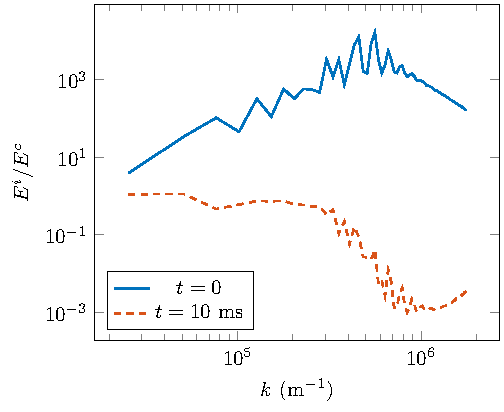
\includegraphics[width=0.48\textwidth]{ch5_kickit/fig2}
    \centering
    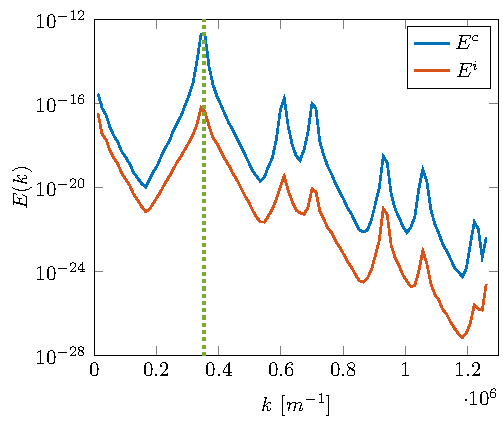
\includegraphics[width=0.55\textwidth]{ch5_kickit/EKcEKi_kick_dt2}
    \caption[Compressible and incompressible energy spectra of a non-rotating condensate directly following a kick.]{Compressible and incompressible energy spectra of a non-rotating condensate directly following a kick. A peak at $k=4\pi/(\sqrt{3}a_o)$ can be seen, which corresponds to the lattice spacing, $a_o$ (indicated by the dashed line), and the smaller, higher energy peaks can be attributed to higher harmonics between nearest and next-nearest neighbours. The incompressible spectrum is much smaller than the compressible spectrum, and thus is neglected for all further analysis. Reprinted from O'Riordan {\textit{et al}.}~\cite{VTX:oriordan_pra_2016}.}
    \label{fig:ekc_eki_novtx}
\end{figure}

The evolution of the nearest neighbour peak in the compressible kinetic energy spectrum during the first 250 ms after the kick is shown in Fig.~\ref{fig:novtx_p5k}$(a)$. It initially oscillates in and out of existence and eventually disperses over a wide range of wavenumbers. Snapshots of the density evolution are given in Fig.~\ref{fig:novtx_p5k}$(b)$, which clearly show that the oscillations correspond to the existence of a transient lattice pattern with several revivals, having the same underlying structure as the optical potential. In fact, the lattice pattern is best formed whenever the main peak in the kinetic energy spectrum goes to zero, i.e.~when the imprinted kinetic energy has been converted into density modulations.

\begin{figure}
    \centering
	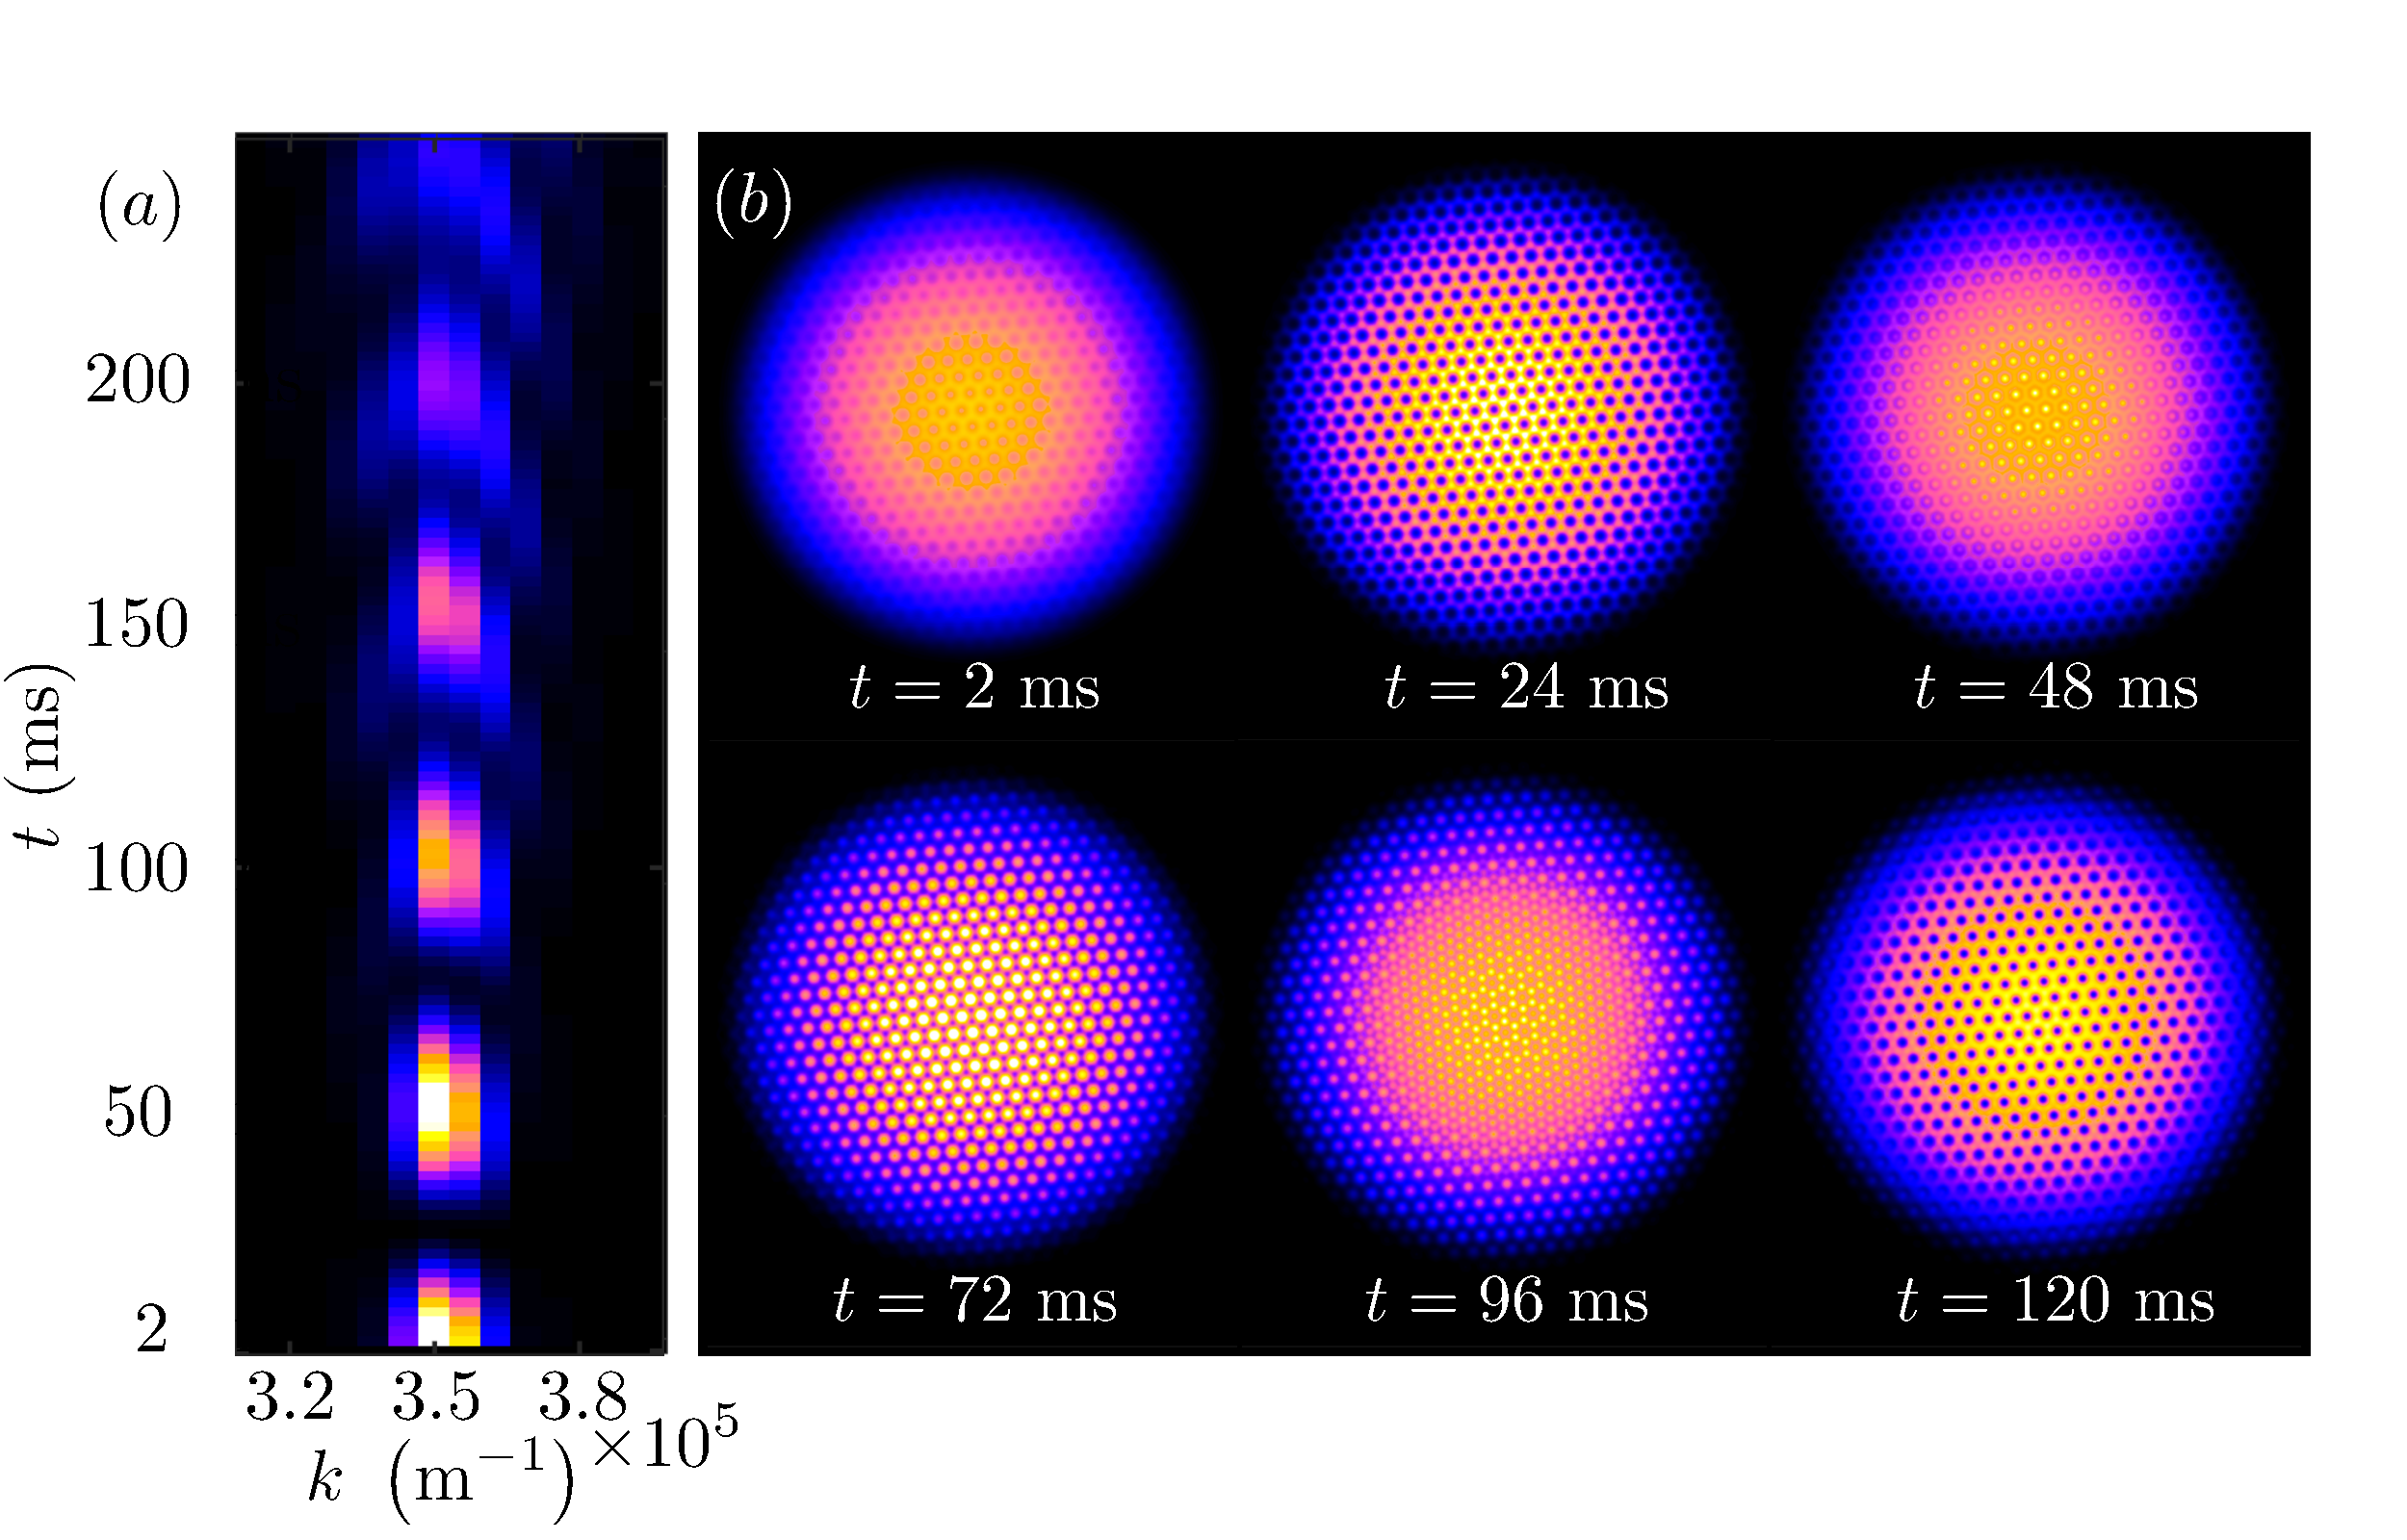
\includegraphics[width=0.80\textwidth]{ch5_kickit/fig3}
	\caption[Effect of kicking on non-rotating condensate.]{$(a)$ Main peak of the compressible kinetic energy spectrum for a kicking strength of $V_0 \approx 1.35\times10^{-2}\mu$. It can be seen to revive, and eventually disperse over a wide range of wavenumbers. $(b)$ Condensate densities at several times during the evolution. A pattern matching the optical potential can be observed to appear and disappear several times over the course of the evolution. Reprinted from O'Riordan {\textit{et al}.}~\cite{VTX:oriordan_pra_2016}.}
	\label{fig:novtx_p5k}
\end{figure}


%######################################################%#################################################################################%############################################################################################################
\subsection{Rapidly rotating condensate}

    Kicking a condensate carrying an Abrikosov vortex lattice with the above optical lattice gives an additional parameter, $\theta_\Delta$, which describes the orientation of the imprinted phonon lattice angle relative to the vortex lattice. We initially assume that the vortex and optical potential lattices have the same lattice constant, $a_v=a_o=a$, which means that symmetry allows for a restriction of the angle to $\theta_\Delta\in[0,\pi/3)$. In the following it can be seen that adjusting $\theta_\Delta$ leads to the appearance of different, transient super-structures in the condensate density. If $\theta_\Delta=0$ (see Fig.~\ref{fig:moire_density}$(a)$) the kicking imparts kinetic energy at wavenumbers that are already well defined in the lattice. No significant change to the compressible kinetic energy spectrum is observed in this case, apart from small amplitude modulations on the well defined peaks.

	\begin{figure}
        \centering
			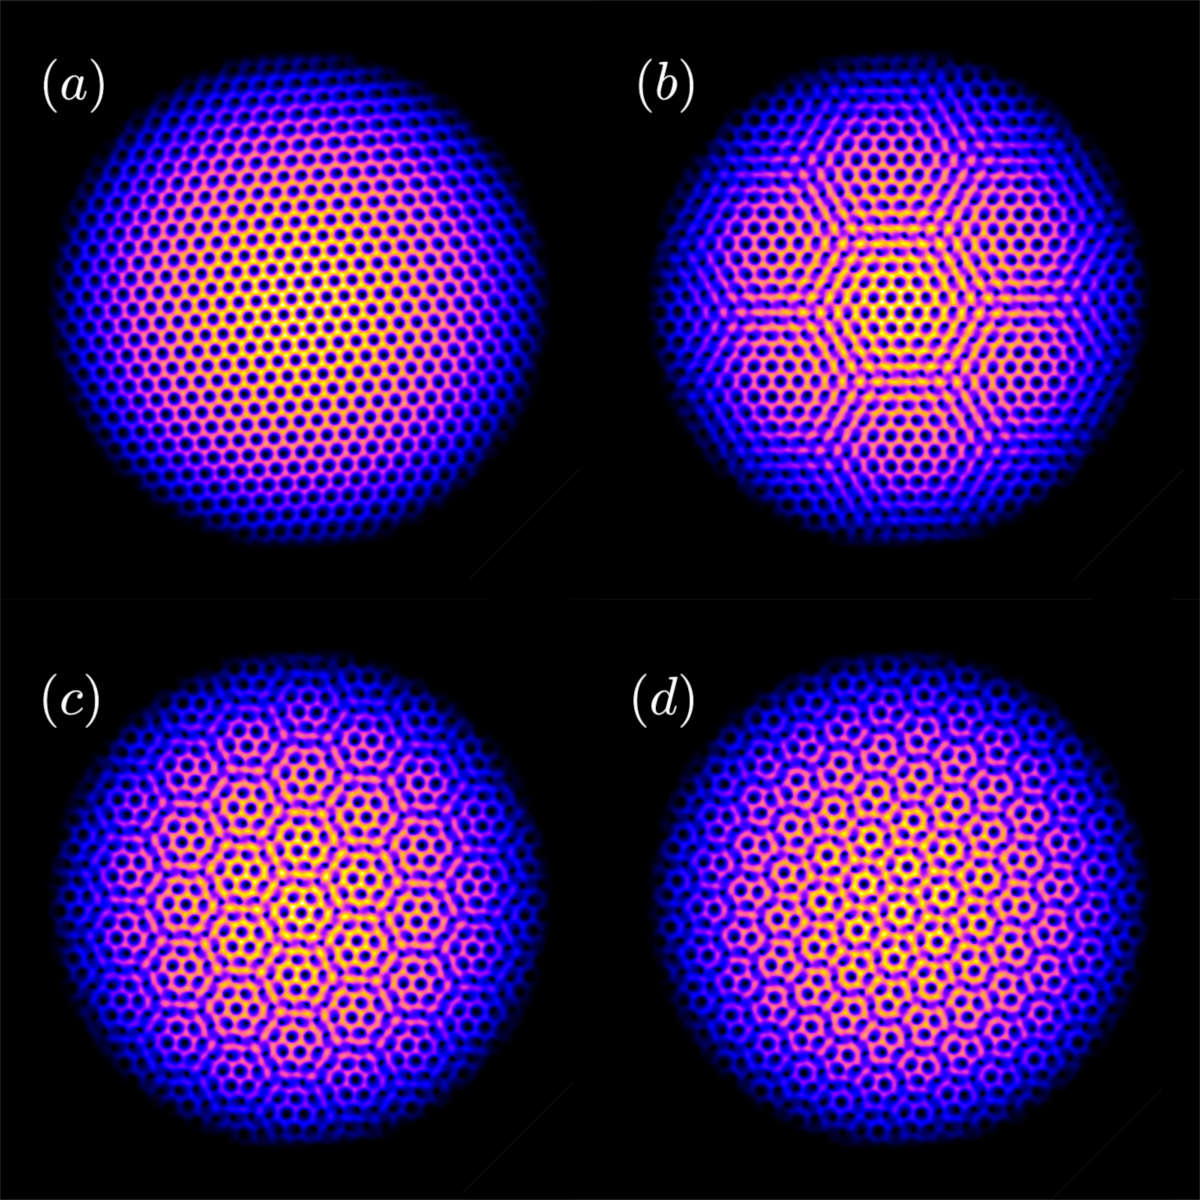
\includegraphics[width=0.55\textwidth]{ch5_kickit/fig4}
			\caption[Effect of kicking on condensate with a large vortex lattice.]{Condensate density at $t=1.4\times10^{-2}$ s for several optical lattice rotation angles. The cell size of the super-lattice structures can be seen to shrink as the angle is increased. The angles for the examples shown are $(a)~\theta_\Delta=0$, $(b)~\theta_\Delta=2\pi/45$, $(c)~\theta_\Delta=4\pi/45$, $(d)~\theta_\Delta=2\pi/15$. Reprinted from O'Riordan {\textit{et al}.}~\cite{VTX:oriordan_pra_2016}.}
			\label{fig:moire_density}
		\end{figure}

    However, if the angle between both lattices is finite, and not an integer multiple of $\pi/3$, superlattice structures appear after a short time (see Fig.~\ref{fig:moire_density}$(b)$-$(d)$), which have a structure cell size that decreases for increasing values of $\theta_\Delta\in[0,\pi/6]$ and beyond which increases for larger values until the misalignment angle reaches the lattice symmetry point again at $\theta_\Delta=\pi/3$. These structures are transient, and several revivals can be observed before the condensate settles back into the vortex lattice structure with an increase in the background wavenumber spread, as expected based on kicking the non-rotating condensate. An example of this for a fixed angle is shown in Fig.~\ref{fig:dtheta20_ev}.

	\begin{figure}
        \centering
		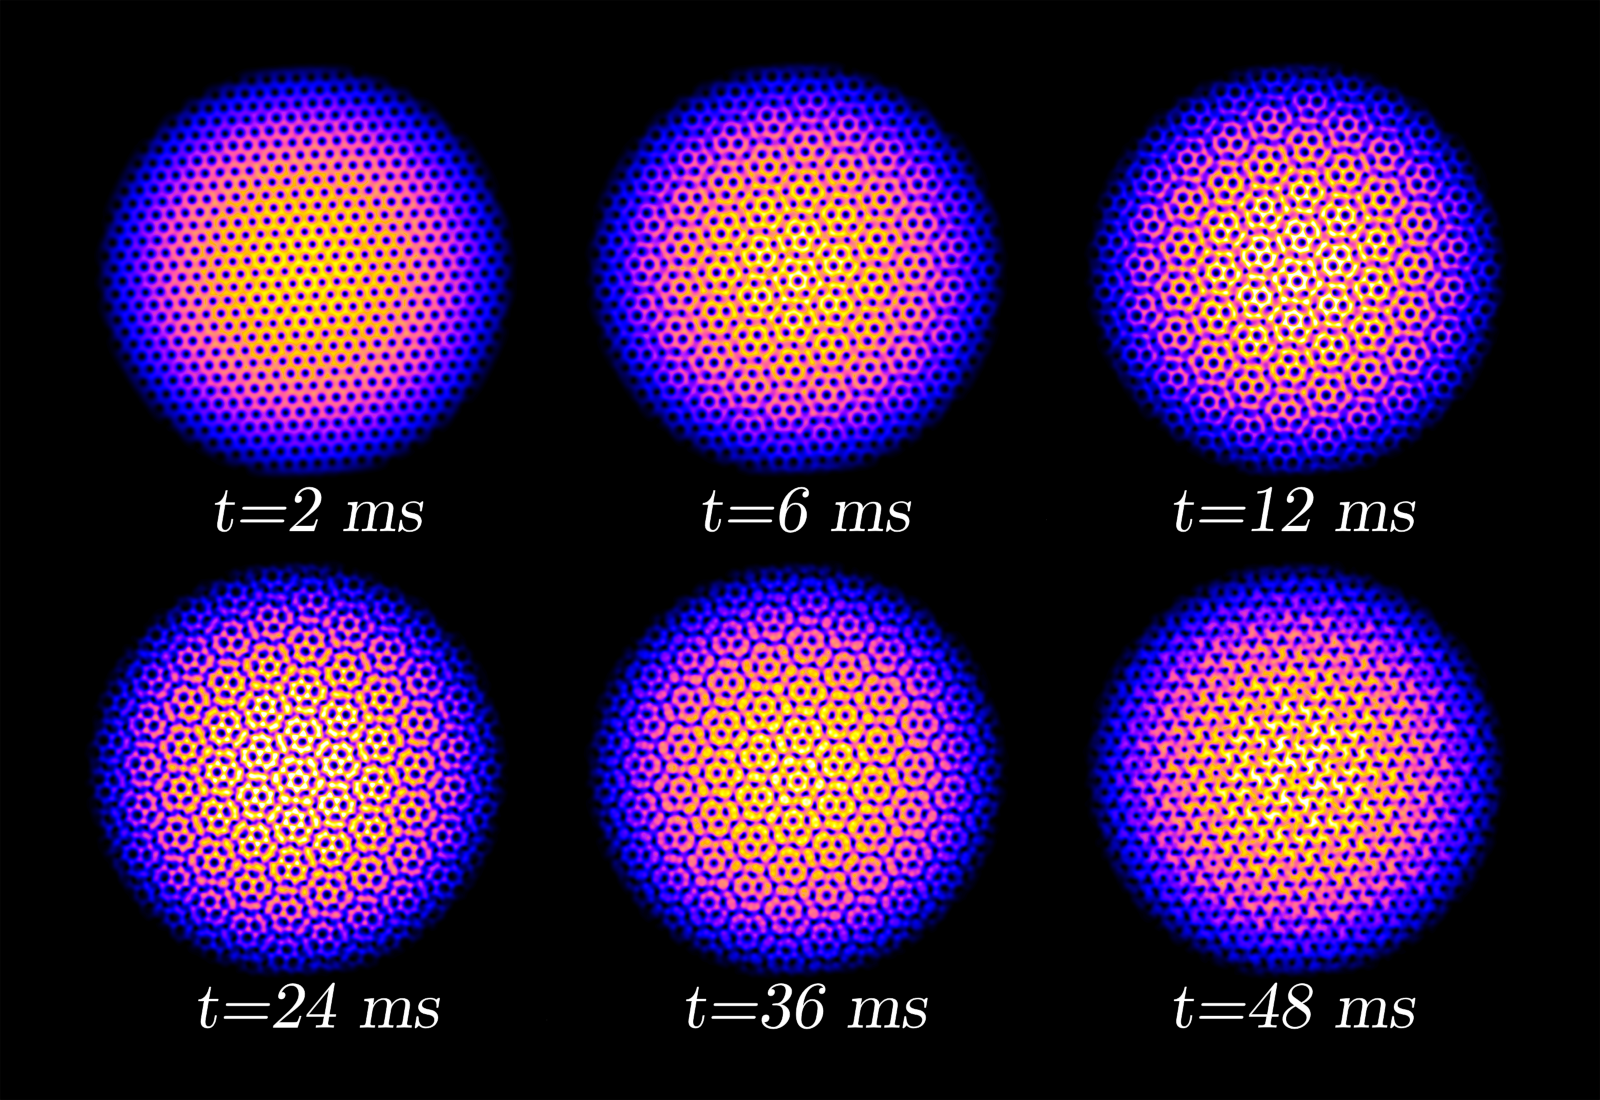
\includegraphics[width=0.55\textwidth]{ch5_kickit/fig5}
		\caption[Oscillation of moir\'e wavelength.]{Condensate density shows visible moir\'e structures upon receiving a kick with $\theta_\Delta=\pi/9$. The appearance and disappearance of a moir\'e structure with wavelength $\lambda_M \approx 2.9 a$ over a timescale of about $50$ ms can be seen. Reprinted from O'Riordan {\textit{et al}.}~\cite{VTX:oriordan_pra_2016}.}
		\label{fig:dtheta20_ev}
	\end{figure}

    To explain the interference patterns observed for misaligning the optical and the vortex lattice, we employ moir\'e interference theory \cite{SS:Hermann_jpcm_2012}. Moir\'e patterns are known to appear when two periodic structures are overlaid while slightly misaligned to each other, and can be calculated from the reciprocal lattice vectors. In all generality, any choice of equidistantly separated reciprocal lattice vectors can be parameterised as
    	\begin{equation}
    		\mathbf{g}_{l} = g_0 \left[ \sin\left( \frac{2\pi l}{\upsilon}+\theta \right),\, \cos\left( \frac{2\pi l}{\upsilon} +\theta\right) \right],
    	\end{equation}
    where $\upsilon$ describes the rotational symmetry of the lattice, $l$ labels the vector direction on the unit circle, $\theta$ is the angle with respect to a chosen coordinate system and $g_0$ is the reciprocal lattice constant. For commensurate and triangular lattices we get $g_0=4\pi/(\sqrt{3}a)$, $\upsilon=6$ and the vector directions are $l=\left[0\dots\upsilon-1\right]$. As only the relative mis-alignement between the vortex and the phonon lattice matters, we choose $\theta=0$ for the vortex lattice and $\theta=\theta_\Delta$ for the optical potential alignment.
    All possible wavelengths that can appear in an interference pattern between two such lattices in position space are then given by
    	\begin{equation}
    		\lambda_{ll'} = \frac{\lambda_0}{|\mathbf{\mathbf{g}_{ll'}|}},
    		\label{eq:InterferenceVectors}
    	\end{equation}
    where
    $\mathbf{g}_{ll'}=\mathbf{g}_{l}^{\text{vtx}}-\mathbf{g}_{l'}^{\text{opt}}$, and
    $\lambda_0 = 4\pi/\sqrt{3}$ for the commensurate triangular lattices. This yields 6 interfering wavevectors, and as a result 6 moir\'e wavelengths. Figure~\ref{fig:moire_higher} shows these resulting interferences in both position and reciprocal space, with the colour indicating the corresponding wavenumbers and wavelengths. The band-like structure of the interferences have contact points at the angle of maximal and minimal alignment of the two lattices, $\theta_\Delta=(j\pi/3,j\pi/6)$ respectively. For a chosen rotation angle between these limiting values, we obtain several wavenumbers, and hence wavelengths. One can see from Fig.~\ref{fig:dtheta20_ev} for $\theta_\Delta = \pi/9$ that a pattern matching the longest wavelength, $\lambda_M= \max[\lambda_{ll'}] \approx 2.9 a$, appears around $t=24$~ms and is clearly the most visible one for the given angle. Shorter wavelengths, while are expected to be present, are hard to discern in this system, and therefore we will concentrate on the lowest wavenumber for the following analysis.

In $\mathbf{k}$-space the shortest $|\mathbf{g}_{ll^\prime}|$ corresponds to adjacent wave-vectors with the smallest $\theta_\Delta$ between them (see inset in Fig.~\ref{fig:moire_lambda_1}). Due to the symmetry of the lattices the most visible structures are therefore given by $\lambda_M=\lambda_{00}$ for $\theta_\Delta\in[0,\pi/6]$ and $\lambda_M=\lambda_{01}$ for $\theta_\Delta\in[\pi/6,\pi/3]$ (see inset of Fig.~\ref{fig:moire_lambda_1}).
While this symmetry assumption no longer holds strictly true after the system has been kicked, it is still fulfilled to a very good approximation during the initial dynamics. One can then obtain the wavelength of the dominating moir\'e structure as~\cite{BIO:Blair_jneur_2007,SS:Yankowitz_natphys_2012}
    	\begin{equation}
    		\lambda_M = \frac{a}{2\sin(\eta/2)},
    		\label{eqn:moire_size}
    	\end{equation}
    where $\eta=\min(\theta_\Delta,\frac{\pi}{3} - \theta_\Delta ) $  (see Fig.~\ref{fig:moire_lambda_1}).
These super-structures become observable when the wavelength becomes smaller than the radius of the condensate, which for the chosen parameters is $\lambda_M \approx 11a$ and which corresponds to an angle $\theta_\Delta \approx \pi/36$.
One can see from Fig.~\ref{fig:moire_lambda_1} that once the relative angle is increased beyond this value the structure sizes shrink to a minimum value at the point of complete misalignment, $\theta_\Delta=\pi/6$, giving $\lambda_M\approx 1.93\,a$, and increase again up to the point of symmetry. Beyond this point the behaviour starts over, due to the symmetry of the lattice. Note that in principle the above procedure can be carried out for square or other optical lattice geometries.

\begin{figure}
    \centering
    %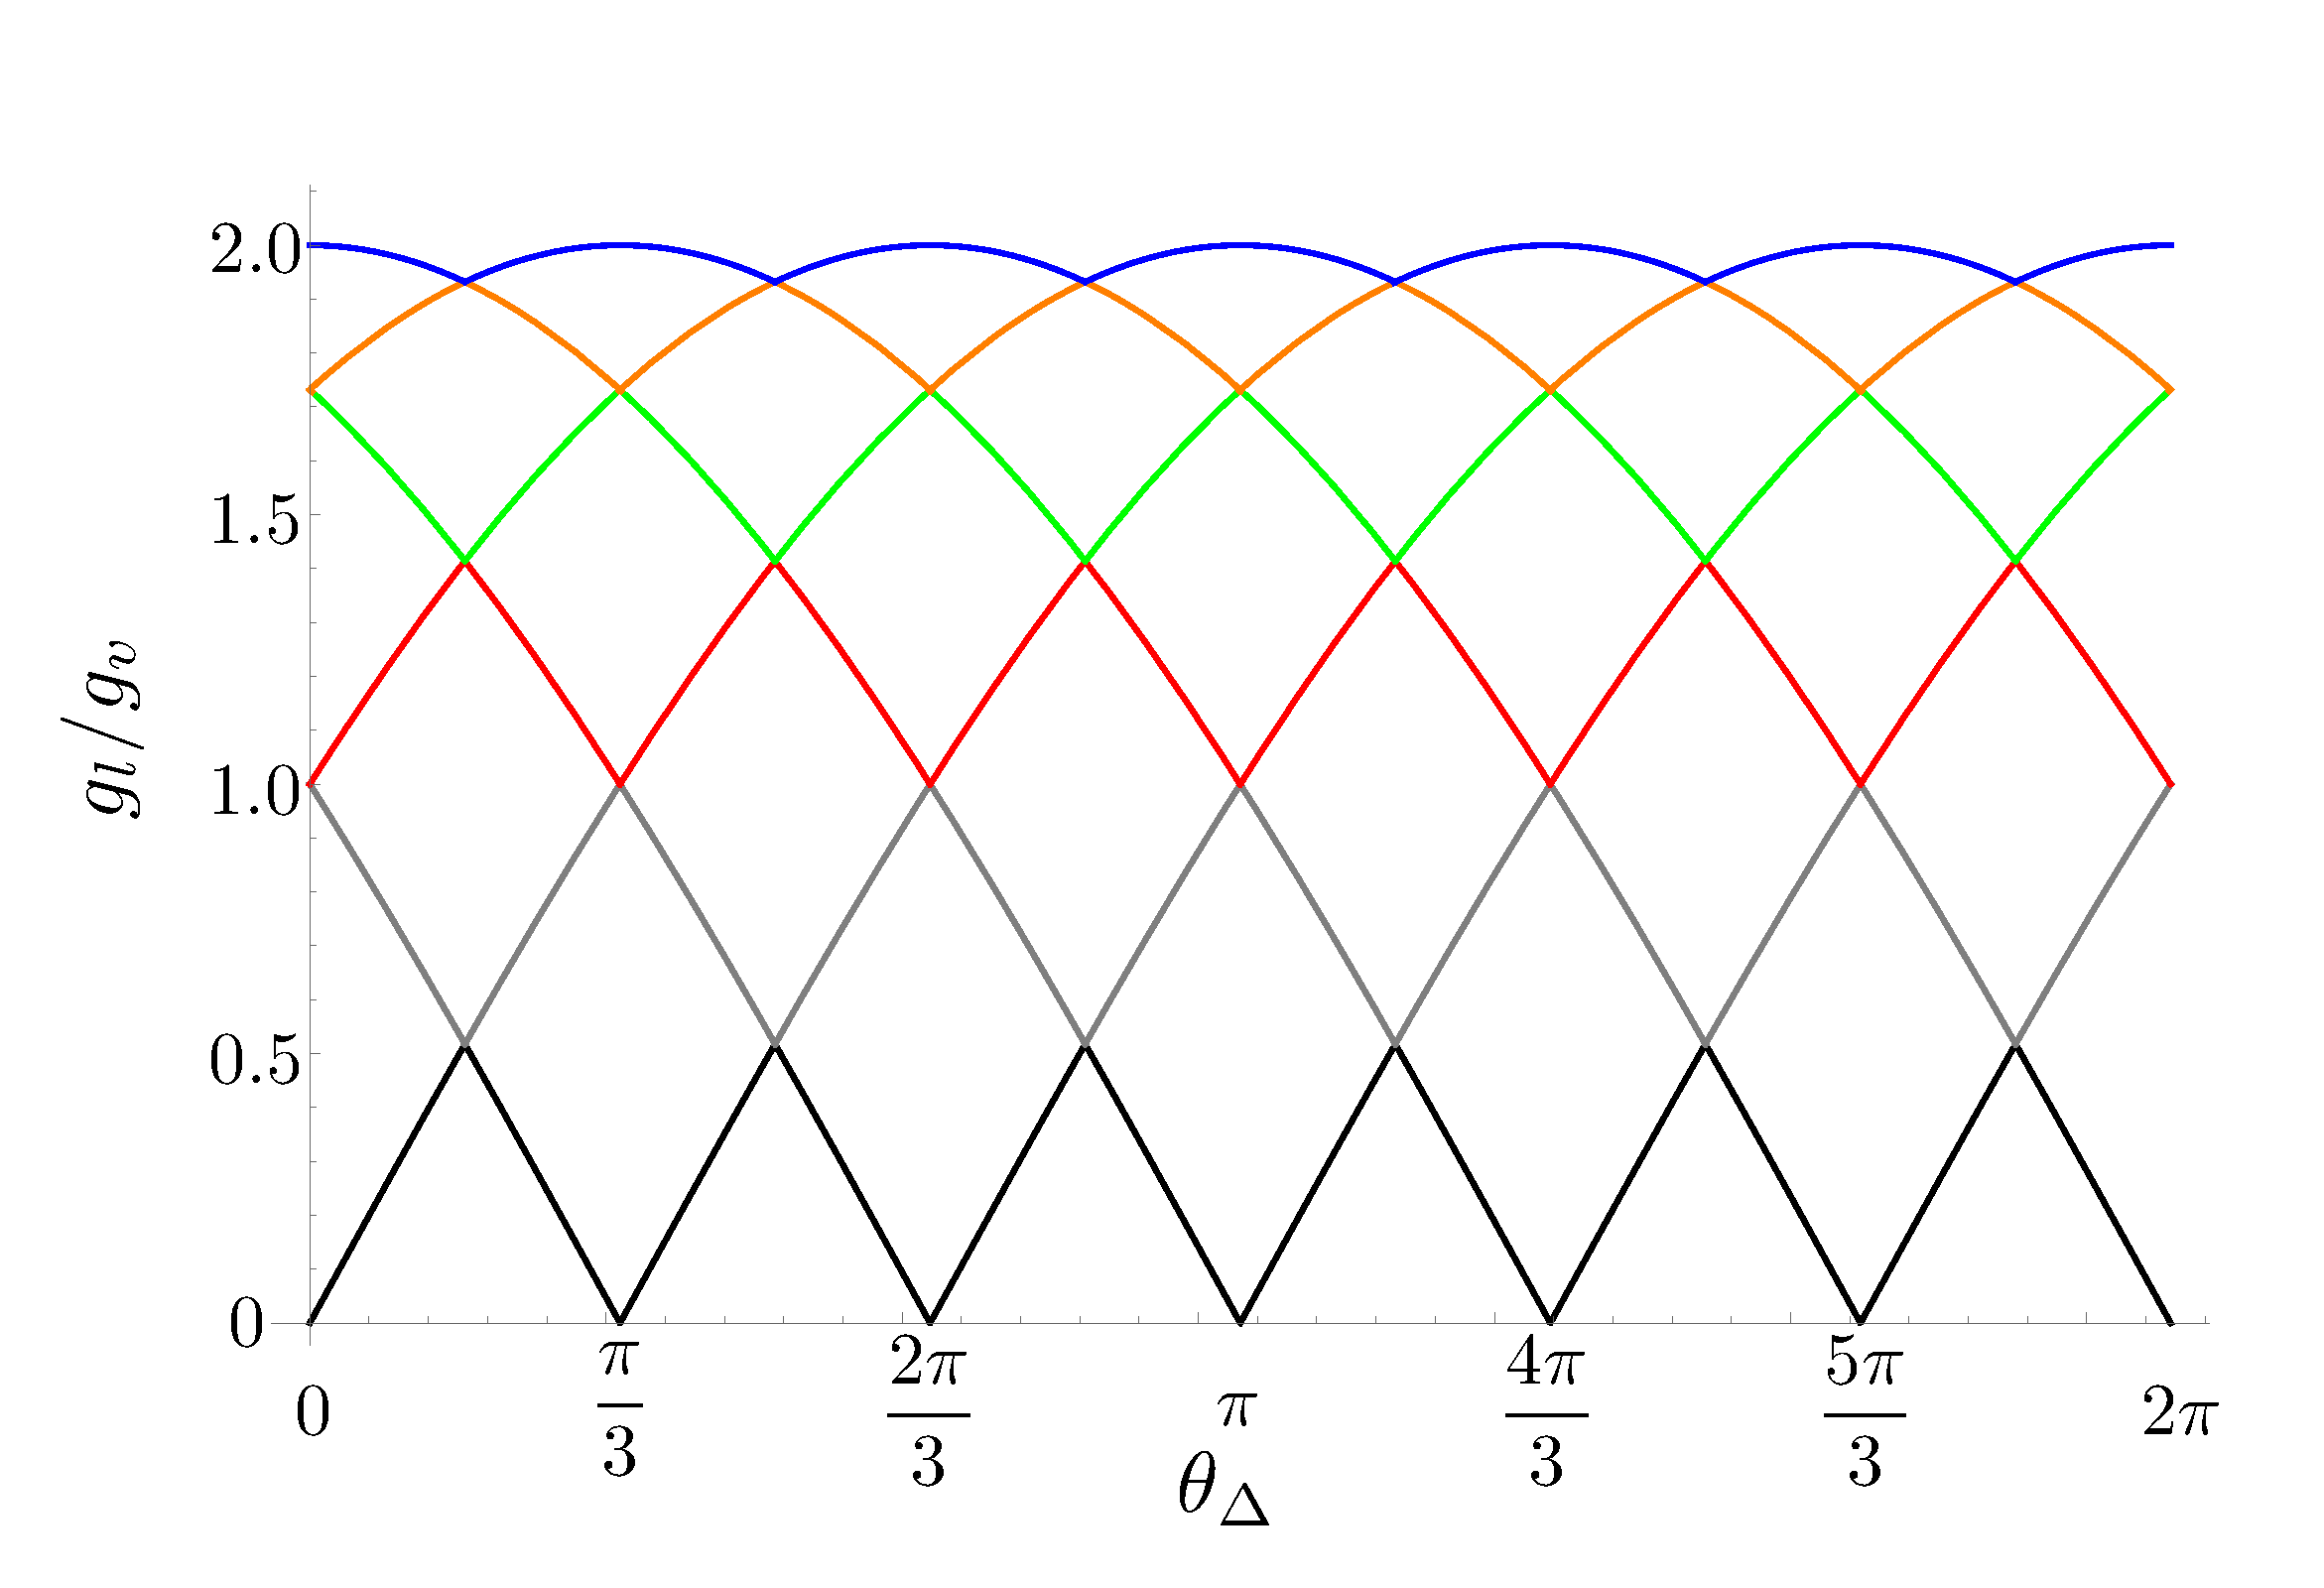
\includegraphics[width=0.48\textwidth,page=1]{ch5_kickit/Moire_lattice_BEC_HigherK_lambda}
    %\includegraphics[width=0.48\textwidth,page=2]{ch5_kickit/Moire_lattice_BEC_HigherK_lambda}
    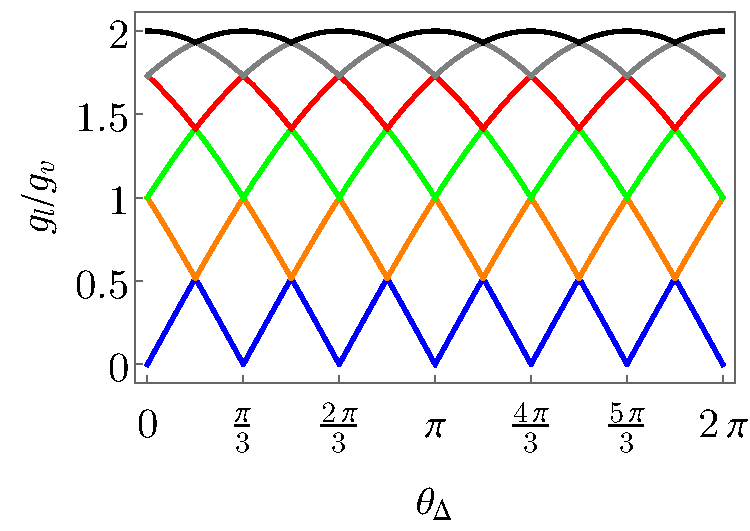
\includegraphics[width=0.48\textwidth]{ch5_kickit/HigherK_k}
    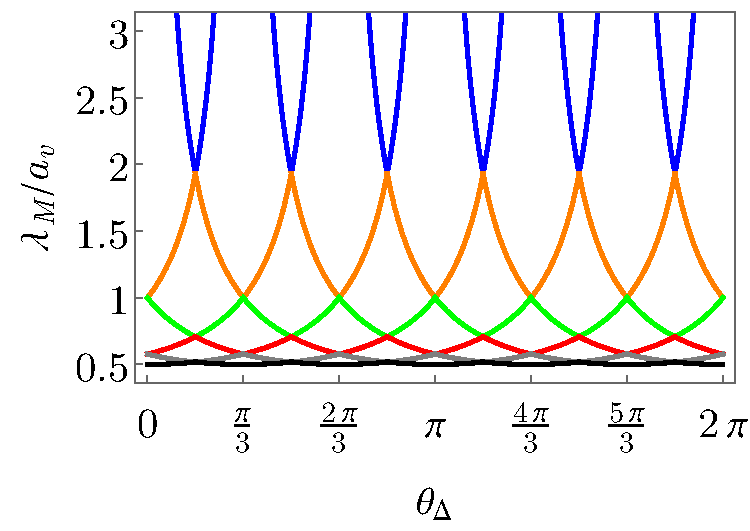
\includegraphics[width=0.48\textwidth]{ch5_kickit/HigherK_lambda}
    \caption[The moir\'e interference pattern in terms of wavenumbers.]{The moir\'e interference pattern in terms of wavenumbers (left) and corresponding wavelengths (right). The resulting wavenumber $g_l$ is normalised by the vortex lattice spacing in reciprocal space $g_v$, and the moir\'e wavelength $\lambda_M$ is normalised by the vortex spacing in position space $a_v$. The lowest lying band in reciprocal space is the main contributor to the visible moir\'e interference patterns, corresponding to the largest wavelength (both in blue). Higher orders are shown for the reciprocal and the corresponding position space, with the higher modes only visible between the beats of the lowest wavenumber moir\'e interferences. Colours correspond between wavelengths and wavenumbers.}\label{fig:moire_higher}
\end{figure}

\begin{figure}
    \centering
	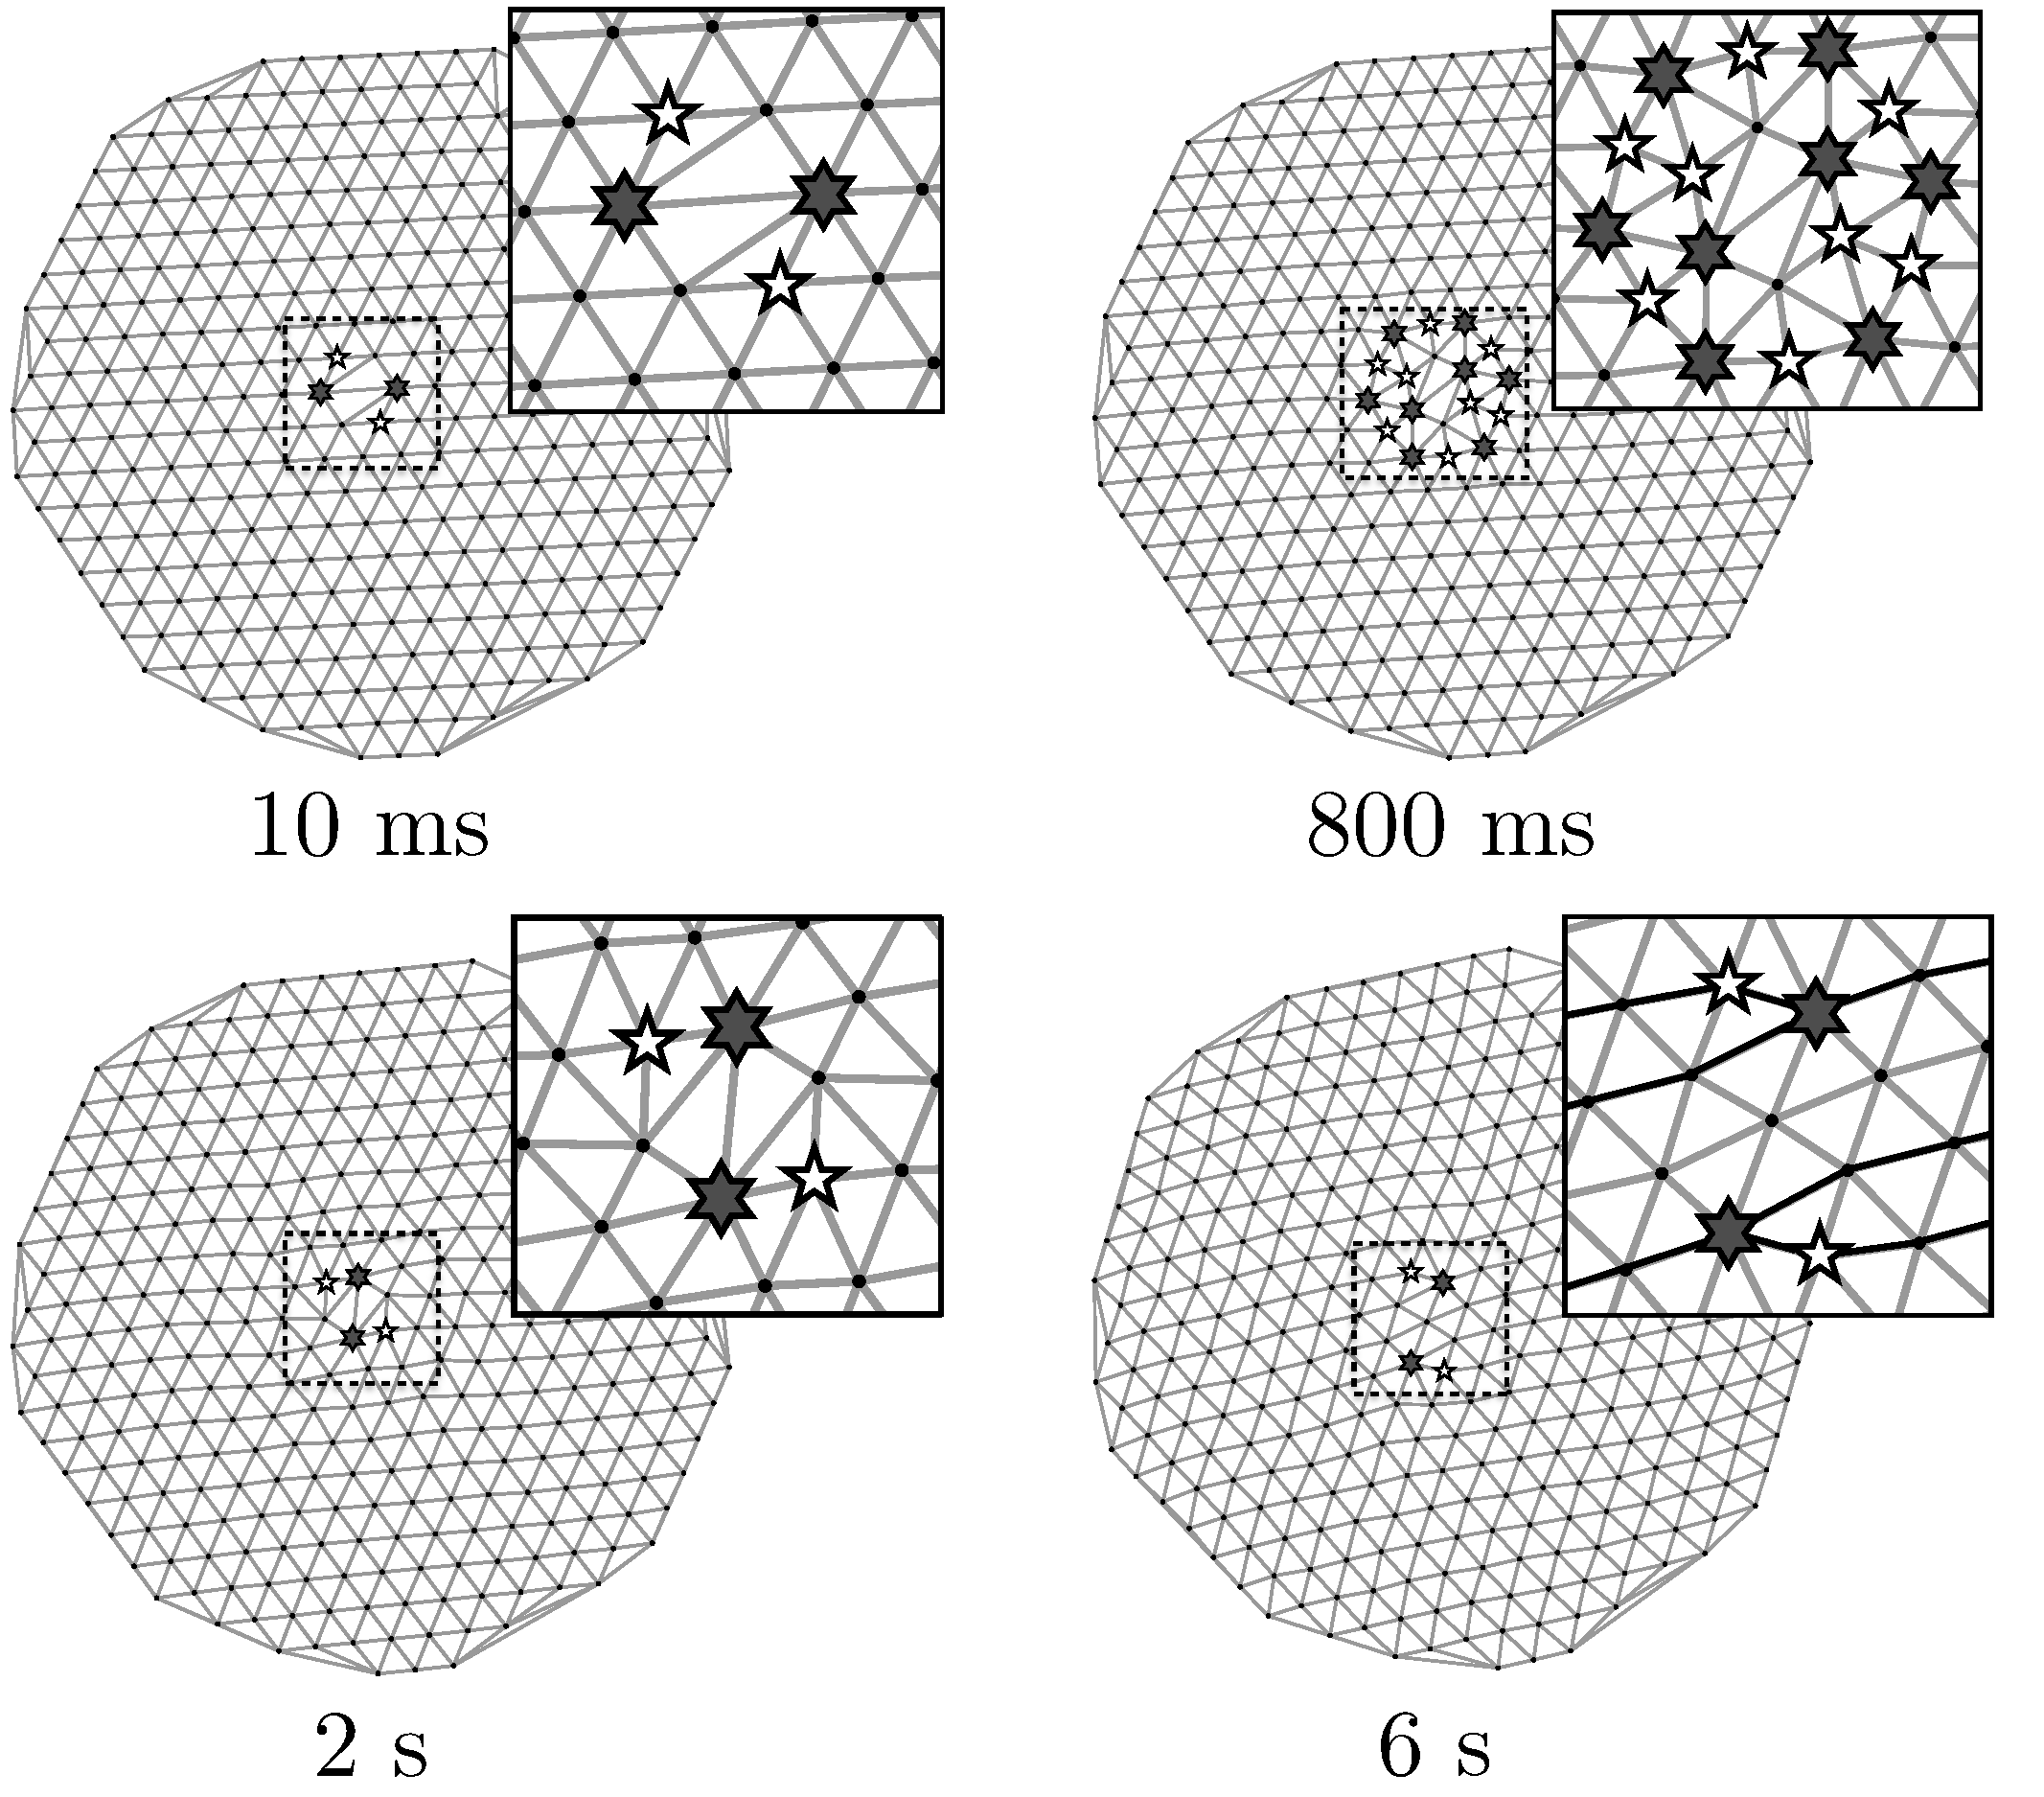
\includegraphics[width=0.55\textwidth]{ch5_kickit/fig6}
	\caption[Size of the resulting moir\'e super-structures as a function of the relative angle between the vortex and optical lattice.]{The dashed green line indicates the condensate radius. Inset: The different vectors in $\mathbf{k}$-space of the two lattices, with the optical lattice rotated by an angle $\theta_\Delta$. The $\mathbf{g}_{ll'} = |\mathbf{g}_l - \mathbf{g}_l'|$ vectors defining the dominant moir\'e wavelength are those for which the enclosed angle is smallest. Reprinted from O'Riordan {\textit{et al}.}~\cite{VTX:oriordan_pra_2016}.}
	\label{fig:moire_lambda_1}
\end{figure}

    The appearance of the moir\'e vector in $\mathbf{k}$-space can be confirmed from the numerical simulations by looking at the compressible kinetic energy spectra which is given in Fig.~\ref{fig:dtheta_kspec}. Apart from the dominant peaks corresponding to the underlying triangular geometry of the Abrikosov lattice, which are independent of $\theta_\Delta$ (straight lines in Fig.~\ref{fig:dtheta_kspec}), a number of additional peaks appear. Their position is a function of the misalignment angle and the lowest wavenumber that appears increases its value with increasing $\theta_\Delta$. This is consistent with the moir\'e model and the appearance of density structures of differing size. Furthermore, a symmetric repeat of this structure about the $\theta_\Delta=\pi/6$ point is also visible, which corresponds to the $\pi/3 - \theta_\Delta$ lattice vector component. The minimum wavelength observed agrees with the theoretically determined minimum value of $\lambda_M\approx 1.93\,a$ and all other values over the range of observed angles. Note that for the higher harmonics at larger wavenumbers similar behaviour exists and is also covered by the moir\'e model.

    To better observe the wavenumbers in the spectra, one can remove the background lattice spectrum. Corresponding to the systems shown in Fig.~\ref{fig:dtheta_kspec} this is given in Fig~\ref{fig:dtheta_kspec_backg}, with the peaks at $t=0$ removed. In this instance, lower wavenumber interference patterns are more easily visualised, with a slight enhancement of higher orders. We can also observe the appearance of secondary interference patterns across low to high wavenumbers, though visibility quickly diminishes approaching higher wavenumbers. It should be noted that given sufficient time the higher order wavenumbers can influence the density dynamics, but the system remains dominated by the lowest wavenumber. Due to the coupling between adjacent modes in the system, all interference patterns become hard to discern after some time. %As the condensate system is finite-sized a refocussing of the interference structures will eventually take place. However, the time-scales necessary to examine this were beyond our numerical capabilities.

    %It is expected (but not investigated) that in the long time limit the interference patterns will eventually refocus and reappear. While the newly generated moir\'e interference patterns can also in turn create additional interferences with the background lattices, I will choose to ignore this effect for the reasons mentioned above regarding higher order wavenumbers.

	\begin{figure}
        \centering
		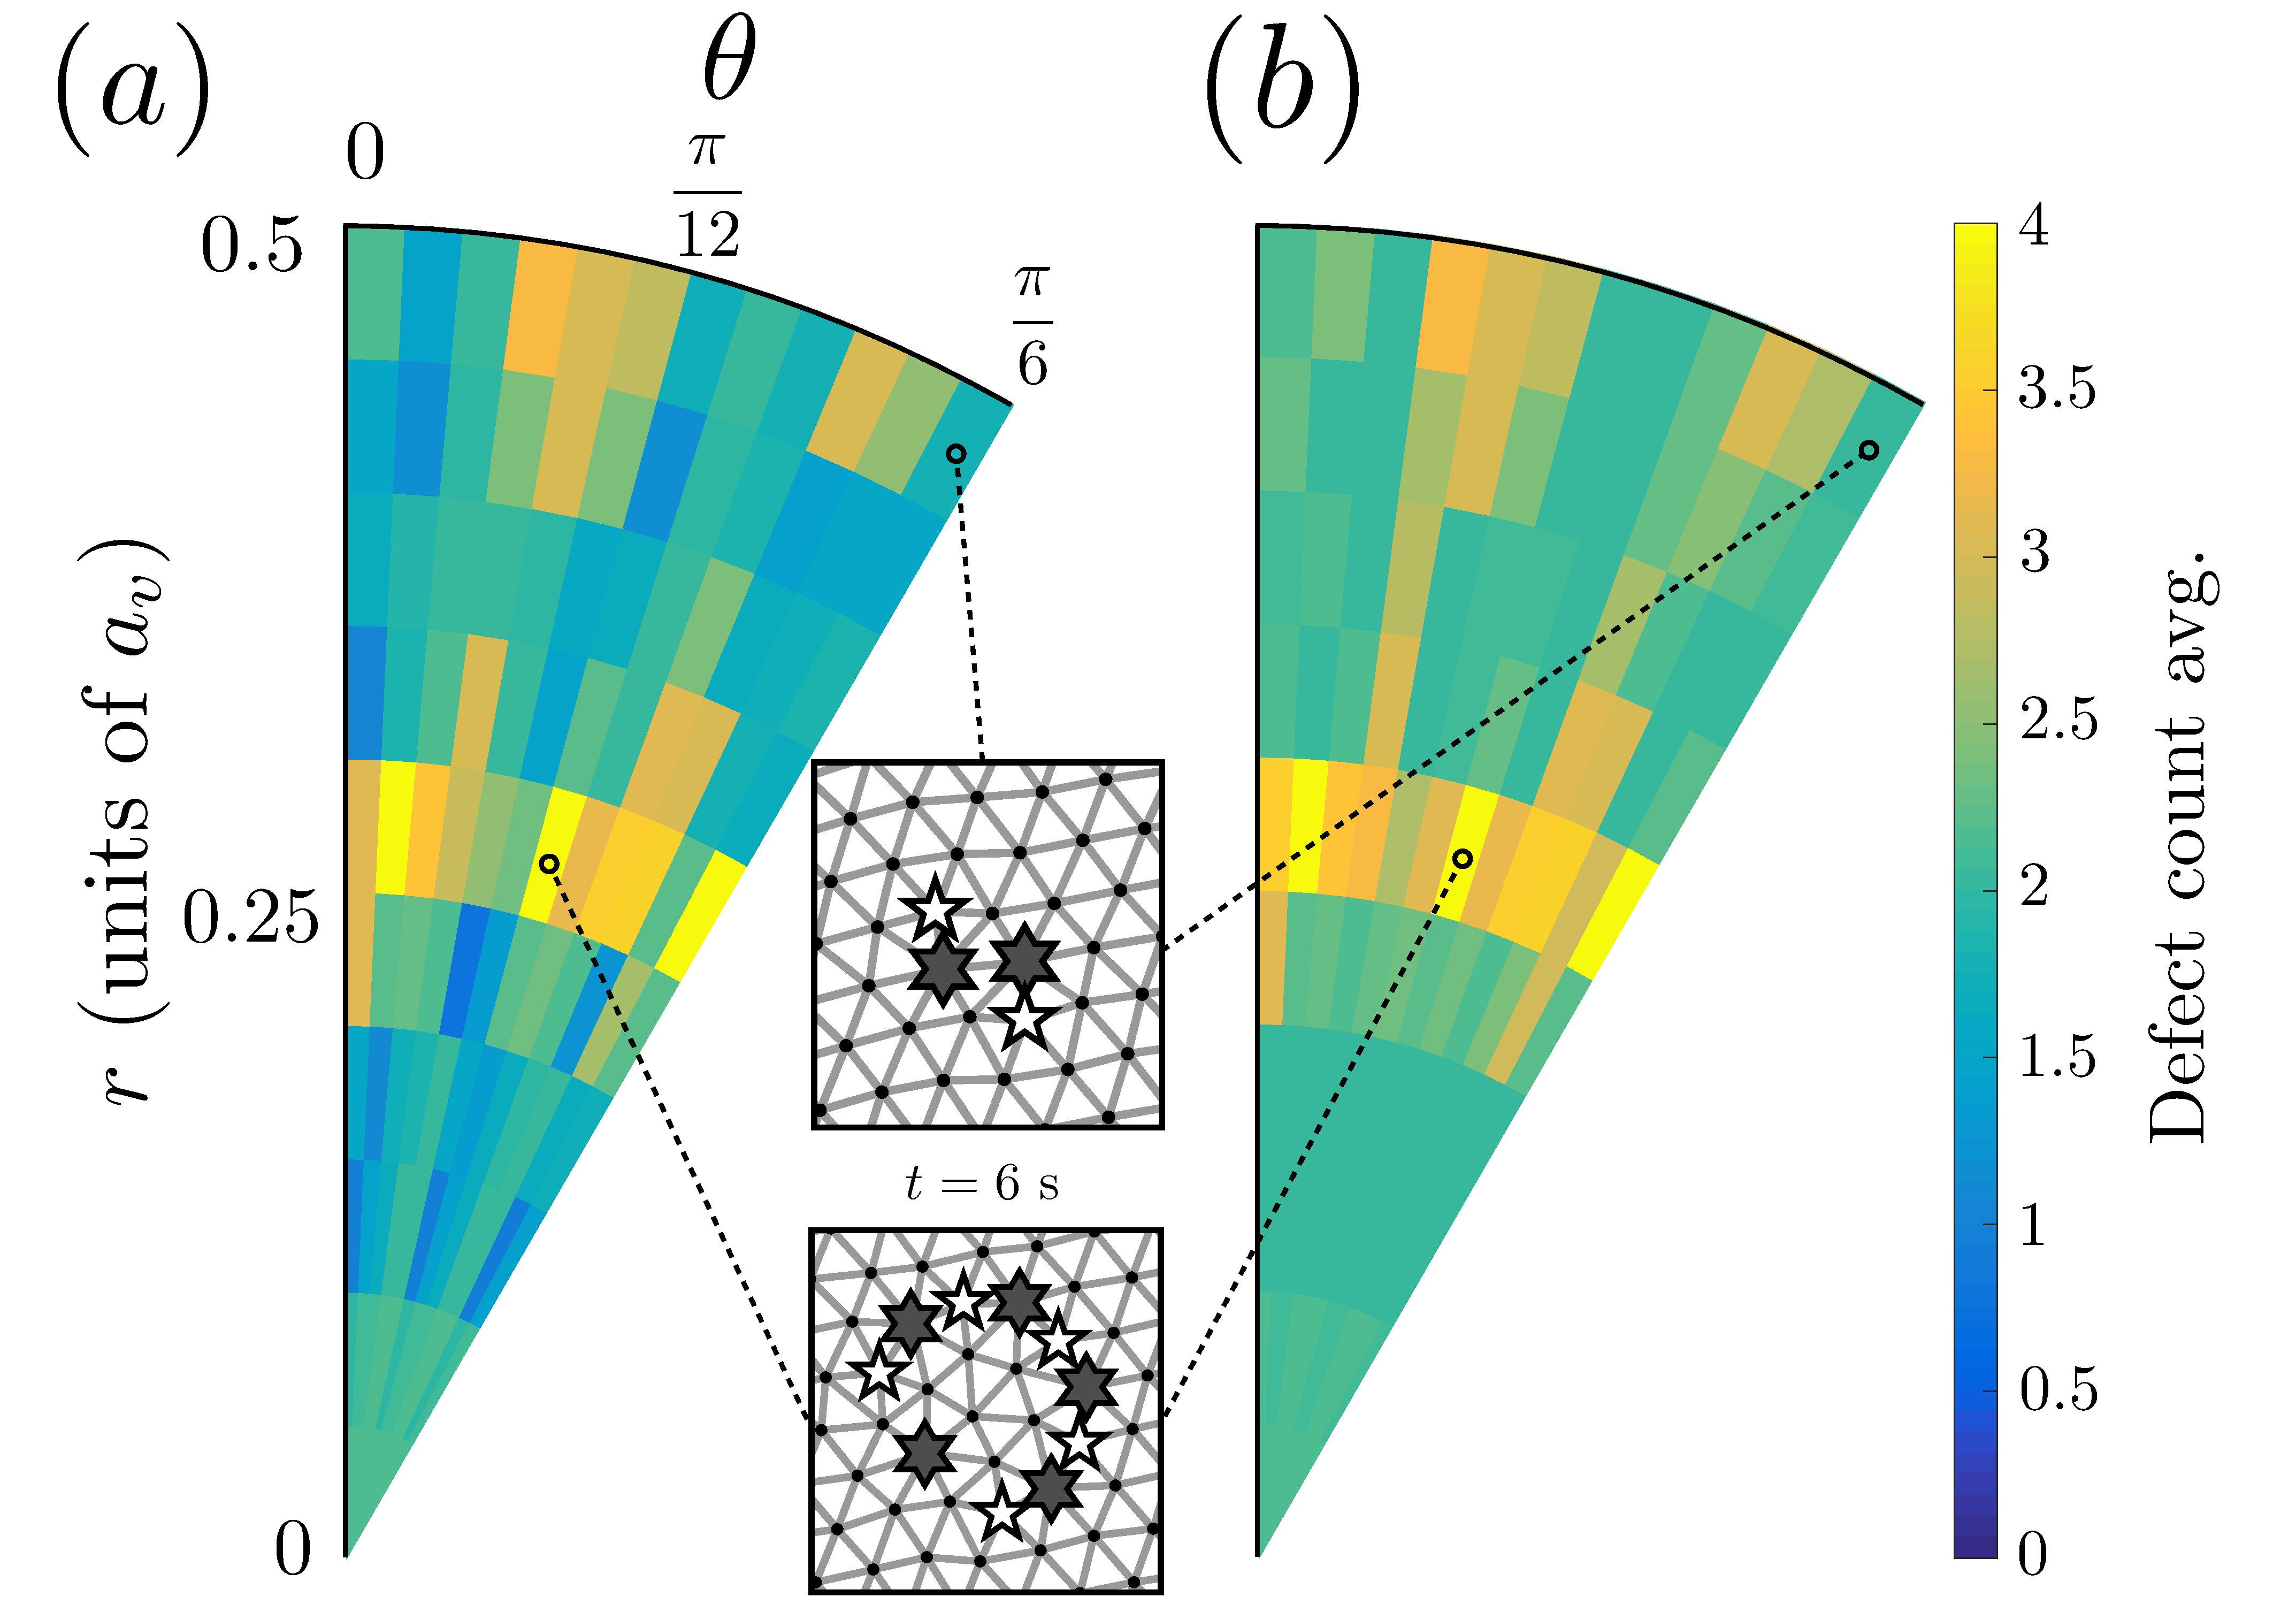
\includegraphics[width=0.65\textwidth]{ch5_kickit/fig7}
		\caption[Compressible kinetic energy spectrum as a function of $\theta_\Delta$.]{Compressible kinetic energy spectrum as a function of $\theta_\Delta$. All values are time-averaged over an interval $t=0$ s to $t=1$ s. The moir\'e peak corresponding to the lowest wavenumber can be seen shifting to larger values for increasing angles and similar behavior is visible for the higher order components. Reprinted from O'Riordan {\textit{et al}.}~\cite{VTX:oriordan_pra_2016}.}
		\label{fig:dtheta_kspec}
	\end{figure}
    \begin{figure}
        \centering
        %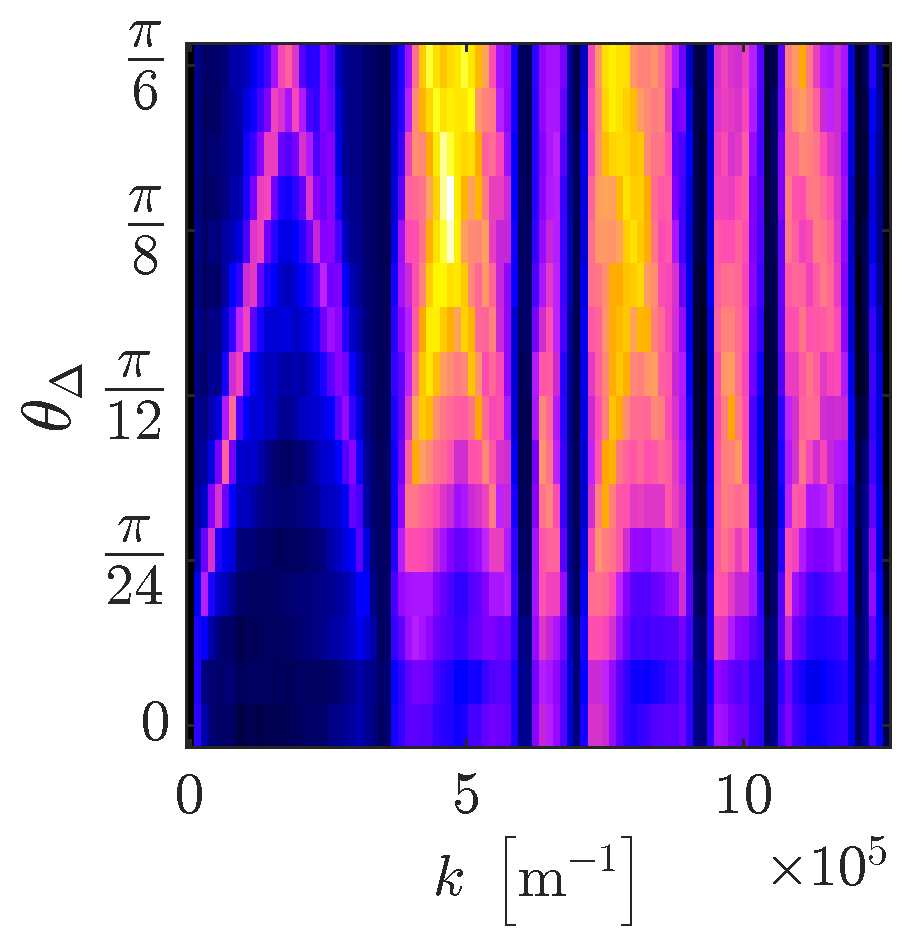
\includegraphics[width=0.5\textwidth]{ch5_kickit/theta_sweep_diff}
        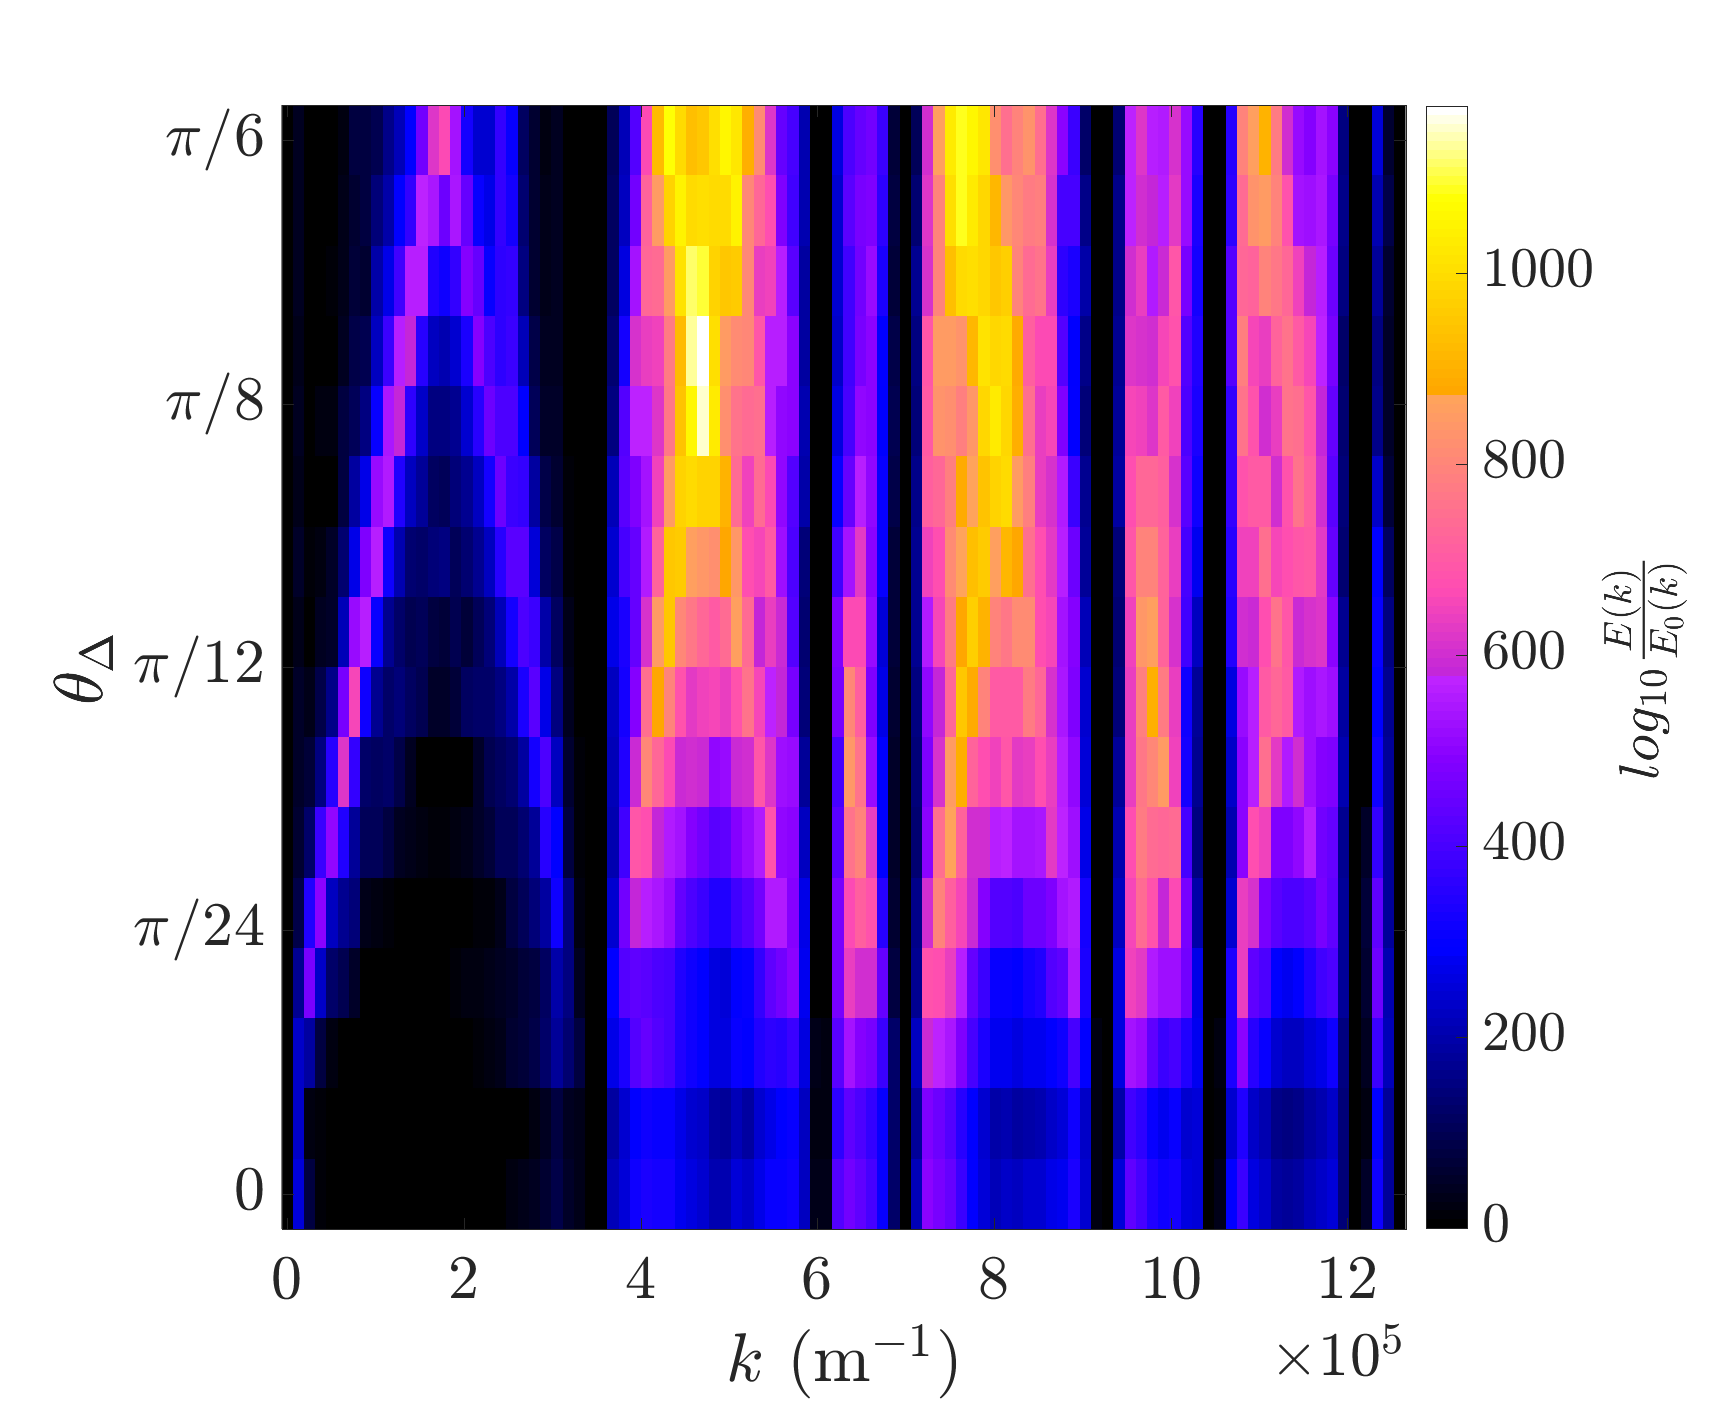
\includegraphics[width=0.65\textwidth]{ch5_kickit/ekc_theta_remove_backg}
        \caption[Compressible kinetic energy spectrum with the background structure removed.]{Compressible kinetic energy spectrum with the structures stemming from the static background removed. The effect of the moir\'e interference pattern for lower and higher modes is more clearly visible compared to Fig. \ref{fig:dtheta_kspec}.}
        \label{fig:dtheta_kspec_backg}
    \end{figure}

    In the following we will briefly discuss what happens for stronger kicking, or when the two lattices are non-commensurate. In the above the strength of the kicking pulse was chosen such that its perturbation only leads to a phase imprinting \cite{Vtx:Dobrek_pra_1999,BEC:Denschlag_science_2000}, with minimal change to the initial density. If one increases the kicking intensity the situation becomes quite different and one can see from Fig.~\ref{fig:kickp20k}$(a)$ that higher order wavenumbers become more strongly excited. This, in turn, leads to modulations of the condensate density at shorter wavelength and an example is shown in Figs.~\ref{fig:kickp20k}$(b)$-$(e)$, with the numerically calculated averaged spectra given in Fig.~\ref{fig:kick_compare_spec}. For fully realistic experimental situations it is necessary to also consider the heating of the condensate once the kicking becomes stronger. However, we do not extend this direction towards stronger kicking strengths in this work.

\begin{figure}
    \centering
	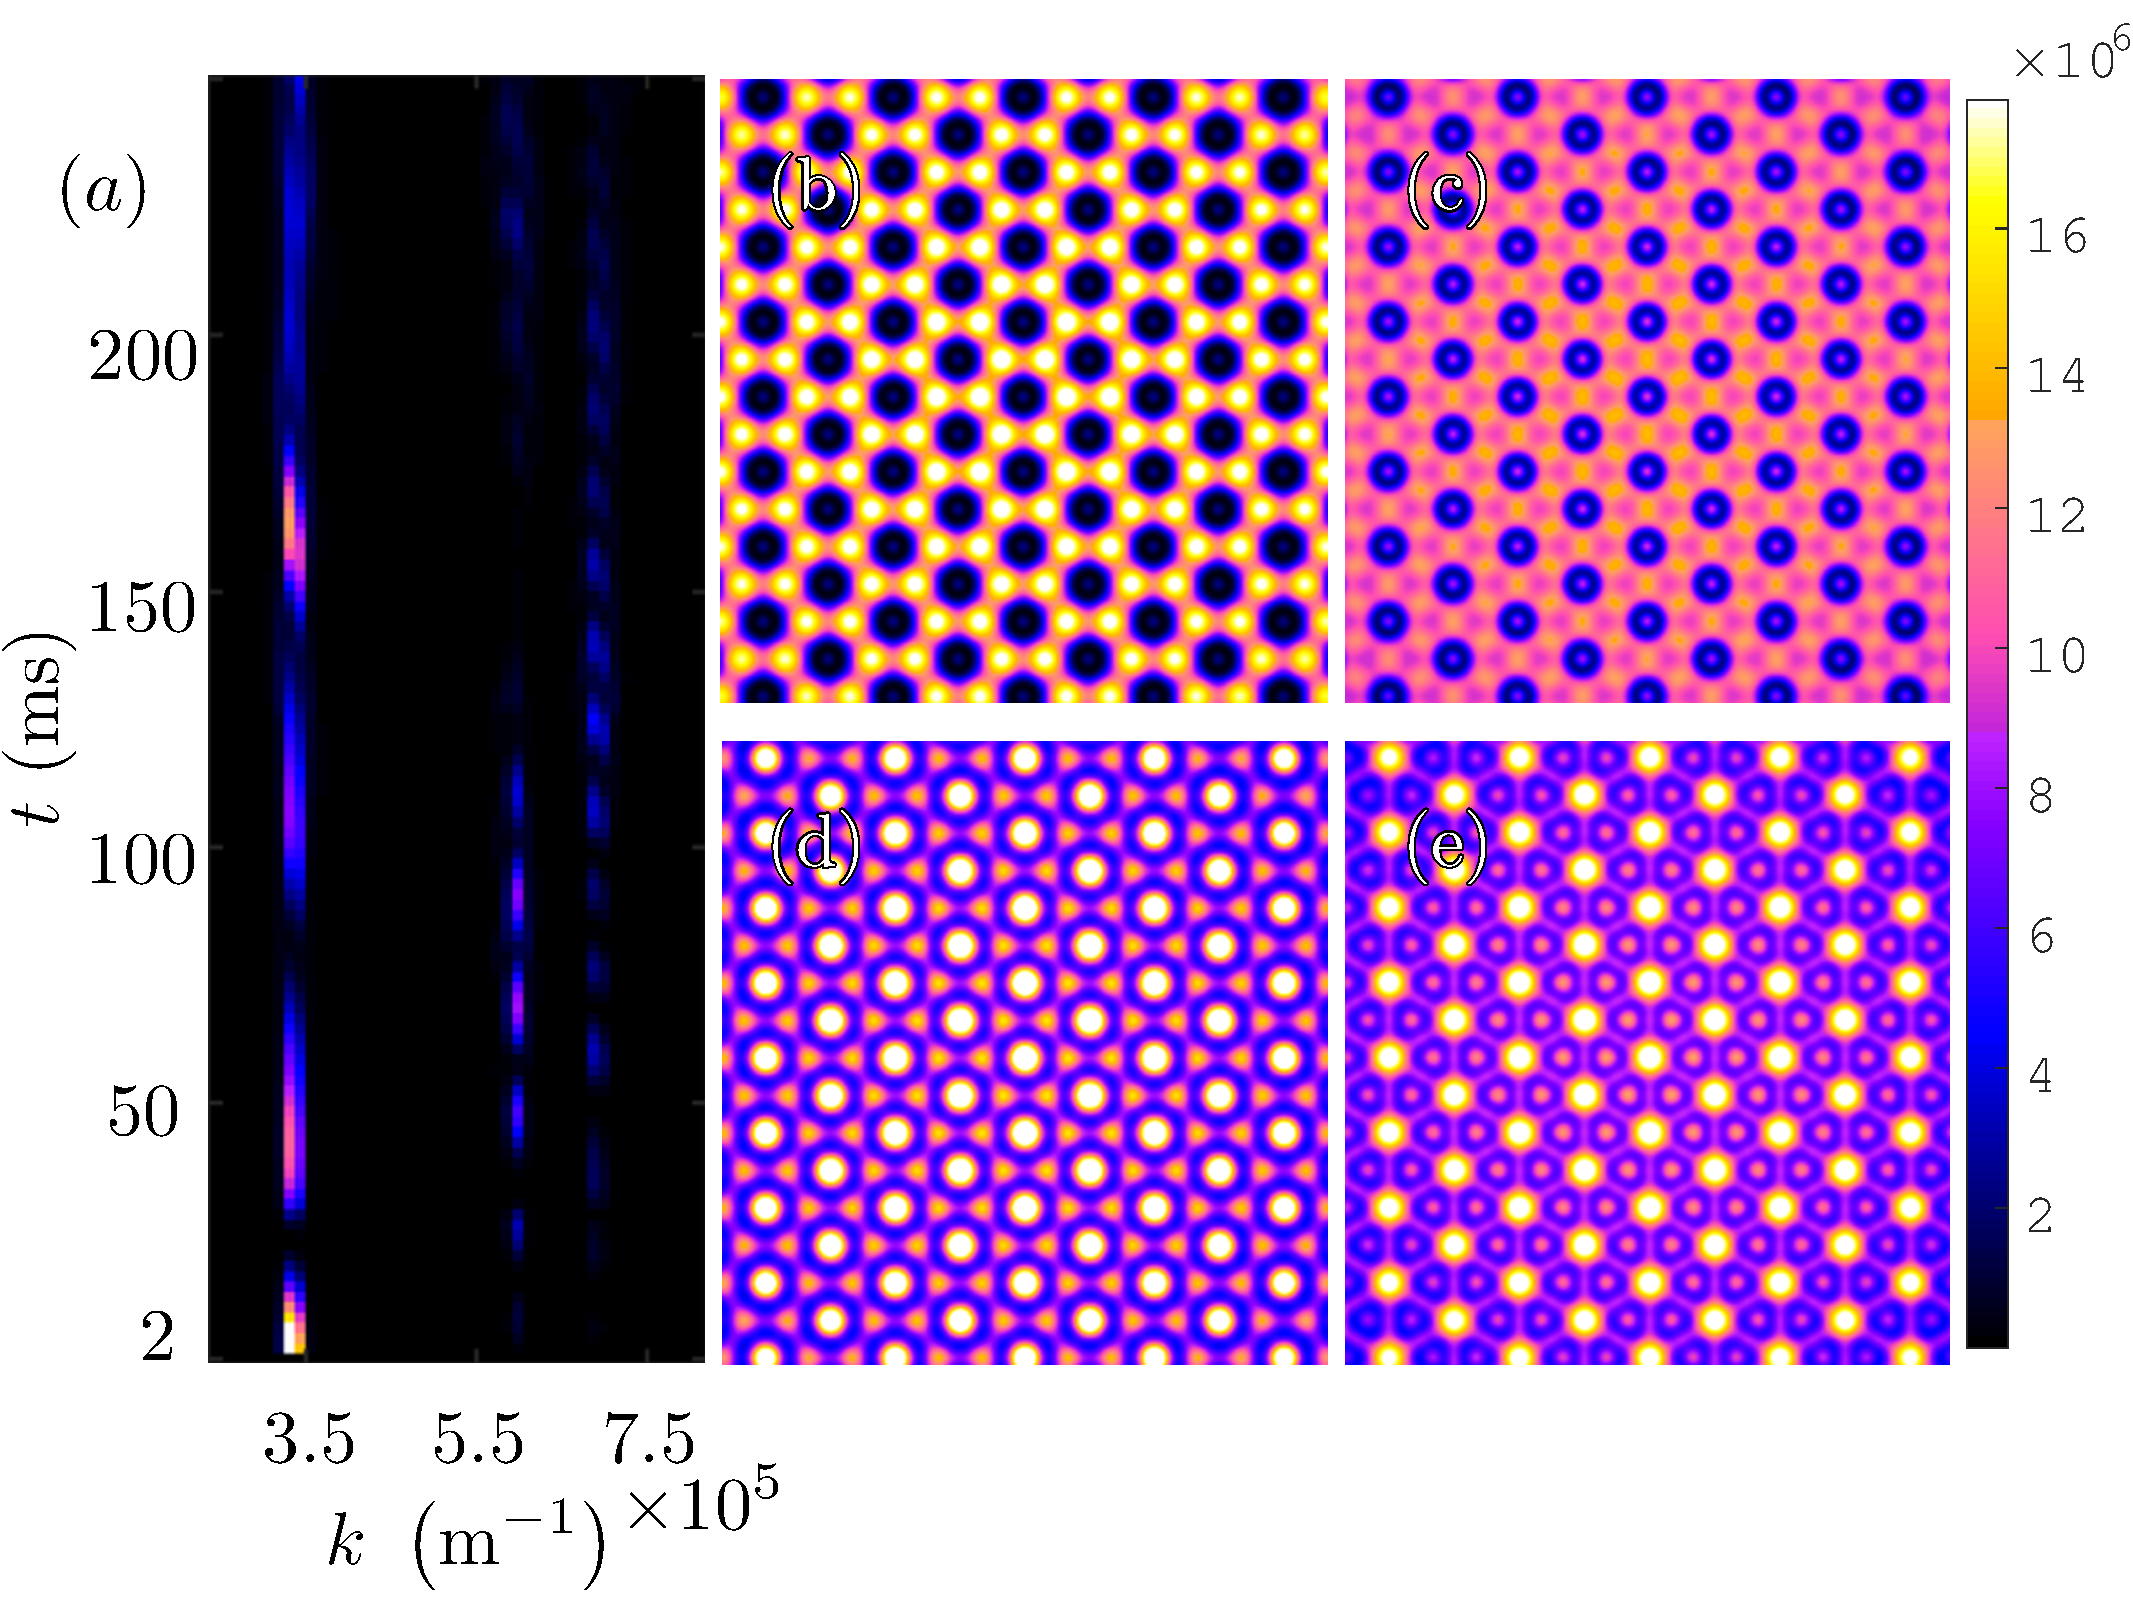
\includegraphics[width=0.75\textwidth]{ch5_kickit/fig8_2}
	\caption[Higher order modes induced by stronger kicking.]{(a) For a kicking strength of $V_0 = 5.4\times10^{-2}\mu$ for a non-rotating condensate higher order modes become non-negligible contributors to the compressible kinetic energy spectrum. This leads to the appearance of higher-order peaks and a different behaviour of the condensate density. Close-ups of the density structures are shown for (b) 24 ms, (c) 36 ms, (d) 56 ms, and (e) 88 ms. Note that the larger structures in these plots are given by the optical lattice constant, $a_o$, which is set to the mean inter-vortex distance for the rapidly rotating condensate. In the presence of vortices this is anticipated to create many additional interferences. Reprinted from O'Riordan {\textit{et al}.}~\cite{VTX:oriordan_pra_2016}.}
	\label{fig:kickp20k}
\end{figure}
\begin{figure}
    \centering
    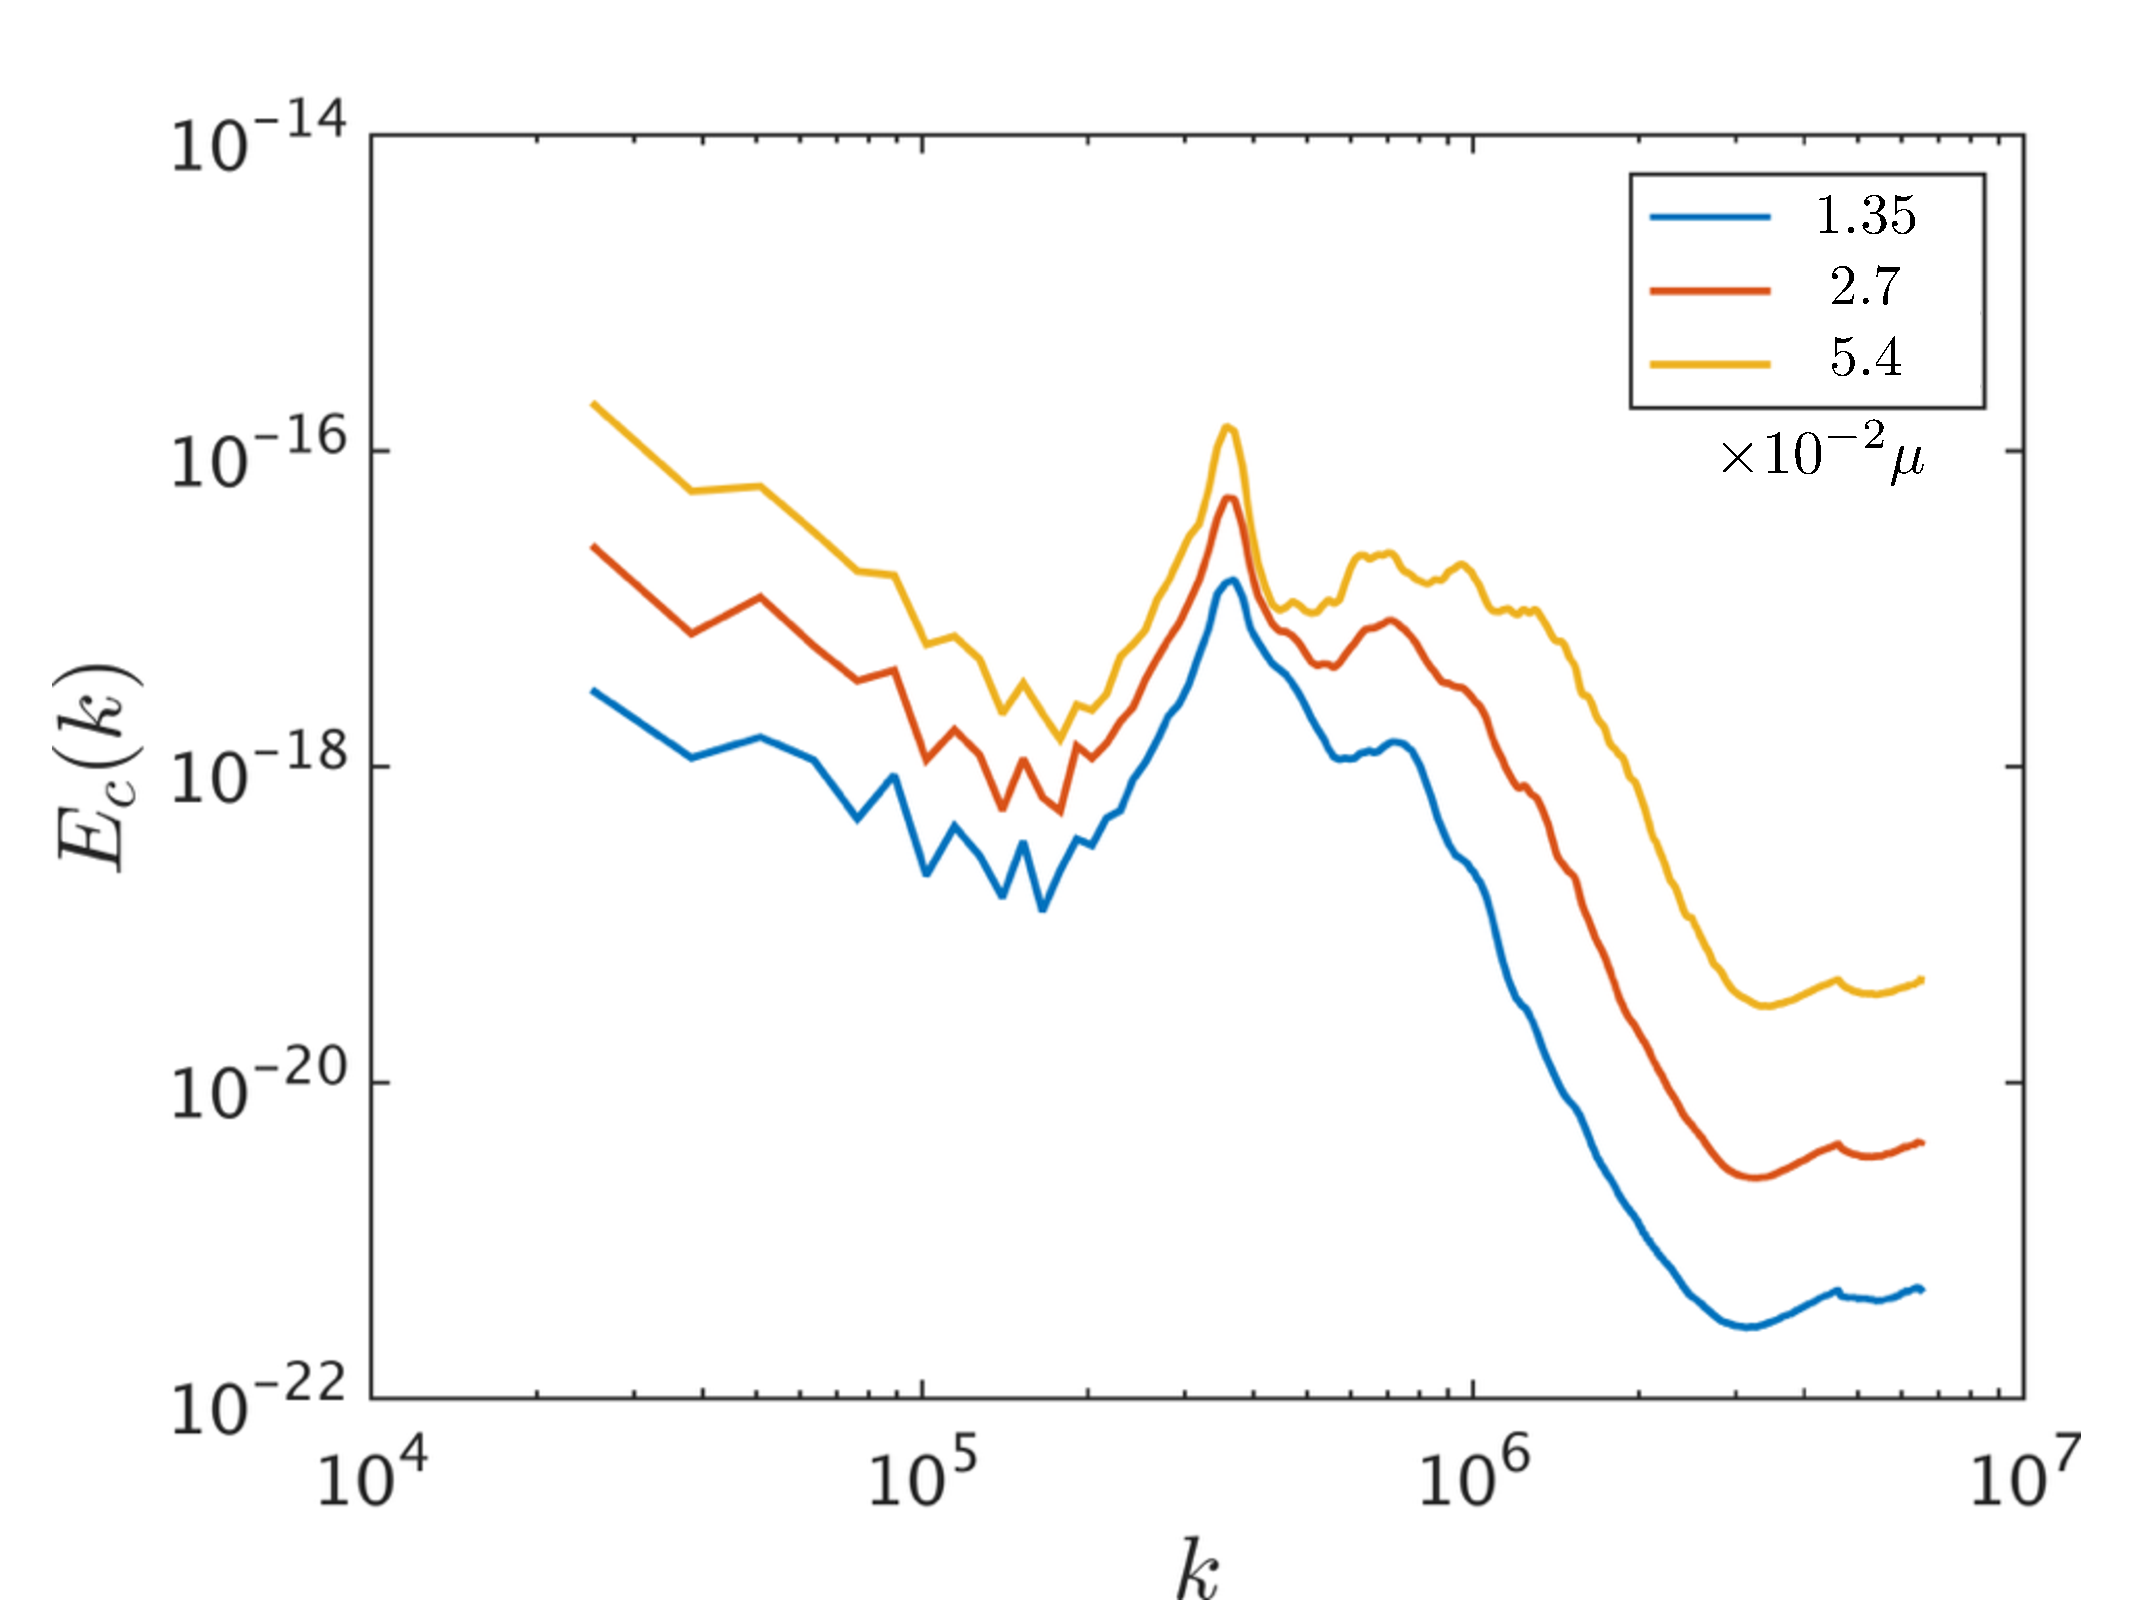
\includegraphics[width=0.49\textwidth,page=1]{ch5_kickit/EKCEKI_novtx_power}
    \includegraphics[width=0.49\textwidth,page=2]{ch5_kickit/EKCEKI_novtx_power}
	\caption[Comparison of kinetic energy spectra for increased kicking strengths.]{For kicking pulses of $V_0 = (1.35,2.7,5.4)\times 10^{-2} \mu$ the kinetic energy spectra show a clear increase in higher order modes being excited for both compressible (left) and incompressible (right) cases with increased kicking strength.}\label{fig:kick_compare_spec}
\end{figure}

    A situation where the optical and the vortex lattice have different lattice constants can be imagined to appear naturally due to experimental uncertainties. Defining $a_o = a_v(1+\epsilon)$ the expression in Eq.~\eqref{eq:InterferenceVectors} can be calculated to be
    \begin{equation}
    	\lambda_M = \frac{a_v(1+\epsilon)}{\sqrt{2(1+\epsilon)(1-\cos\theta) + \epsilon^2}},
    	\label{eqn:moire_size_eps}
    \end{equation}
    which reduces to Eq.~\eqref{eqn:moire_size} for $\epsilon=0$. Evaluating this expression for $\epsilon = (-0.1,0,0.1)$ shows that the largest moir\'e wavelength changes slightly for small values of $\epsilon$, but it remains distinct enough from the higher order wavelengths to stay visible in the evolution (see Fig.~\ref{fig:epsilon}). This ensures that the system examined here is experimentally realistic. For large deviations of the lattice constant, the assumption of the largest moir\'e wavelength playing the dominant role is no longer valid, as many of the interfering wavevectors approach comparable scales.

    \begin{figure}
        \centering
        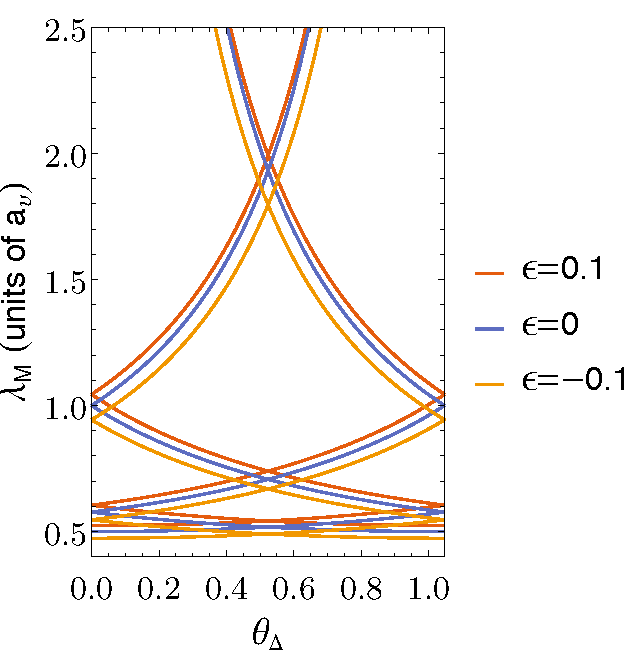
\includegraphics[width=0.5\textwidth]{ch5_kickit/Moire_higherk_epsrange}
    	\caption[Moir\'e wavelengths for imperfect lattice alignment.]{Small deviations for $\epsilon$ can be seen to only lead to minor changes of the induced moir\'e wavelength.}\label{fig:epsilon}
    \end{figure}

\section{Vortex dynamics following a kick}\label{sec:moire_dyn_lattice}
While we have concentrated mostly on the phonon modes of the condensate density it is necessary to also examine the result of kicking on the vortex lattice. Figure~\ref{fig:kickit_traj} shows the densities and trajectories in the co-rotating frame for kicks of $\theta_{\Delta}=\pi (1/60, 1/10)$. Some deviation from solid-body rotation is observed at the edge of the examined vortex region, but the central vortex regions show almost no variation from their ideal lattice positions.
\begin{figure}
    \centering
    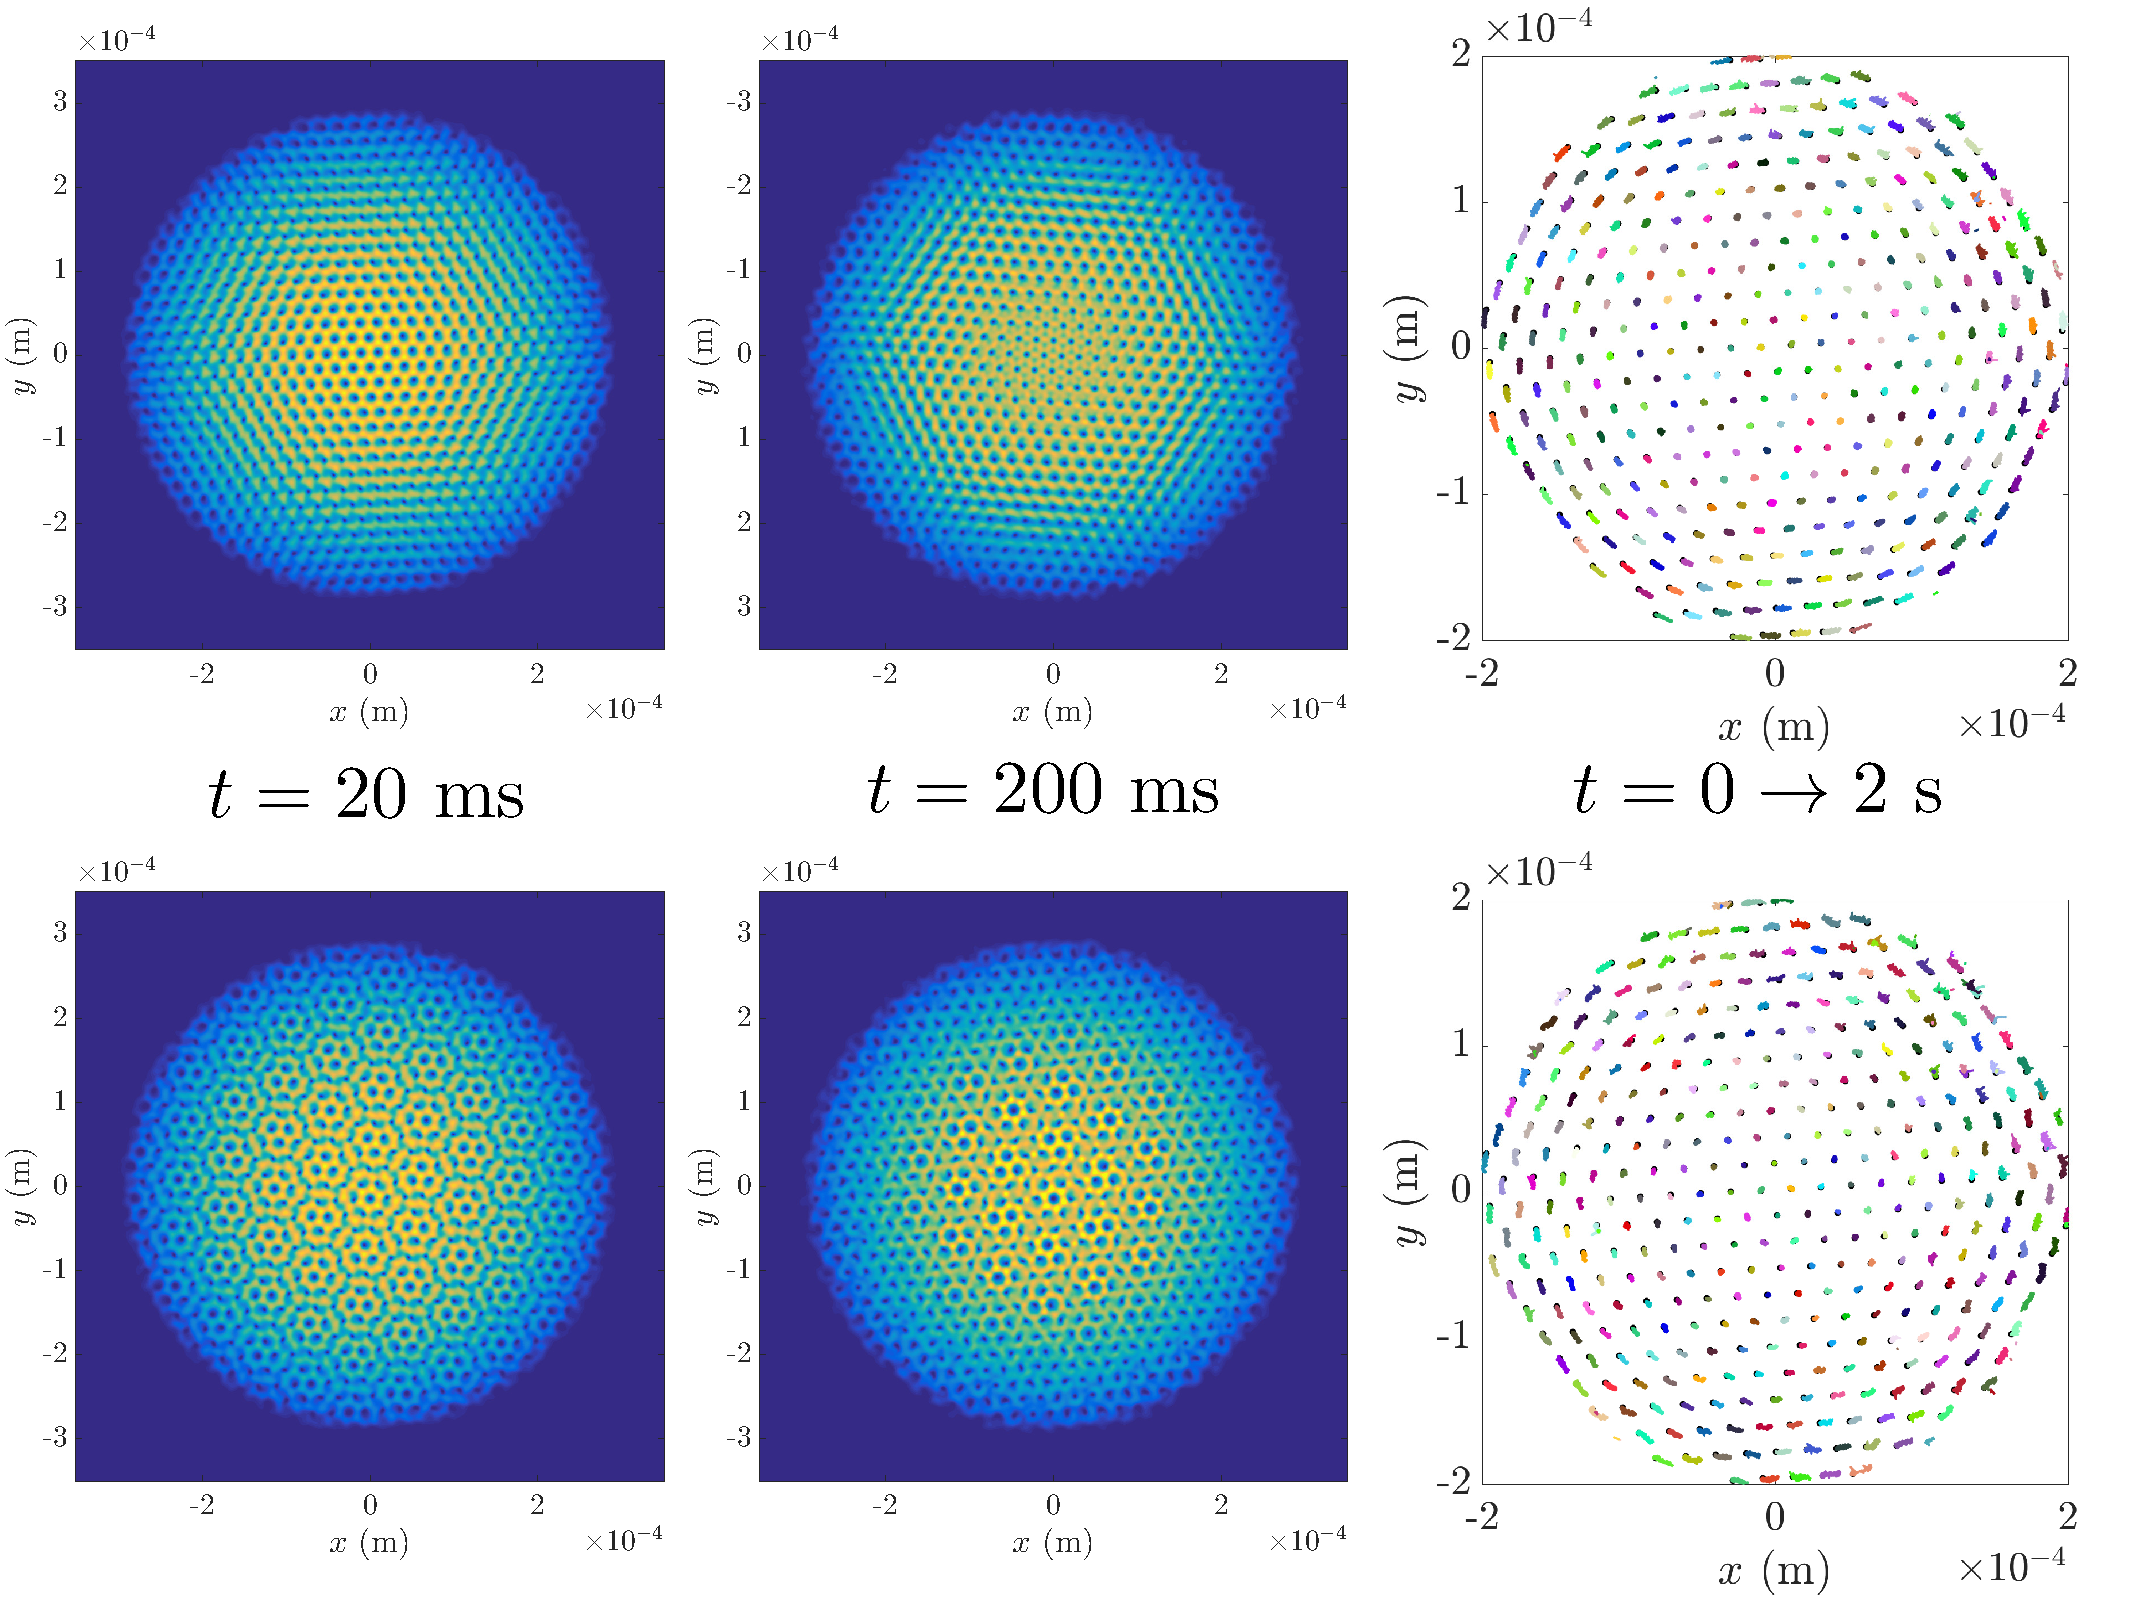
\includegraphics[width=0.9\textwidth]{ch5_kickit/Trajectory_after_kick_theta0_15_3offset}
	\caption[Vortex densities and trajectories following a kick.]{The condensate densities are shown for times $t=(20,200)$ ms, and for $\theta_\Delta = (\pi/60,\pi/10)$ (top and bottom). The resulting trajectories of the vortices show minimal deviation from their initial lattice positions over 2 seconds of time evolution.}\label{fig:kickit_traj}
\end{figure}
Both cases demonstrate the same overall dynamics, with the vortex lattice showing extreme robustness against the phononic perturbances that build following a kick.

\section{Conclusions and outlook}\label{sec:ch5_conc}
The purpose of the previous work was to investigate the effect of a kicked optical lattice potential with a well defined periodicity on a vortex lattice having its own periodic structure. As observed, the kicking had a negligible effect on the vortex positions, with the lattice remaining well defined with near constant spacings, even in the long time limit. The optical lattice kicks solely modified the background density around the vortex cores. One could observe that the vortex lattice remains incredibly stable and strongly resilient to perturbations and modulations in density. Given the stability of the lattice, it can be expected that even for a finite number of kicks, the lattice will remain mostly unbroken. It can also be expected that heating effects would play a role in destabilising the condensate, and to determine any long-term realistic behavior from this system, including the treatment of a non-negligible thermal cloud contribution would be necessary.

The kinetic energy spectra provided a useful tool to investigate the order of the imparted wavenumbers following a kick, and were very closely matched with the results from moir\'e interference theory. The existence of this moir\'e interference effect has some interesting consequences. It can, for example, be thought of as a tool to test the periodicity of a structure that is otherwise too small to be resolved without time of flight. In general, this technique may be used on other types of periodic structures, for example crossed solitons in 2D condensates \cite{BEC:Morgan_soliton_2013}. As optical lattices can offer a large number of free parameters (lattice constant, amplitude, misalignment, geometry, $\ldots$), a full toolbox can be developed from this technique. This could potentially be used for probing condensate systems, applying well-defined structures onto stationary condensates, and for generating the aforementioned interferences in the presence of an underlying periodicity.


While in my thesis proposal the system discussed in this chapter was suggested to investigate delta-kicked chaotic dynamics~\cite{CT:Gardiner_pra_2000}, it became clear very quickly that the robustness of the vortex lattice with respect to realistic kicking strengths did not allow for significant vortex dynamics. Nevertheless, an investigation into periodic kicking is still an interesting (and numerically even more challenging) endeavor. As vortex lattices feature a well-defined rotation rate and 6-fold symmetry, the system rotates to a symmetric position every $\pi/3$. Providing a periodic kick at this rate, would therefore allow the lattice to always have the same alignment angle, at least for an initial number of kick repetitions.
